% This is LLNCS.DOC the documentation file of
% the LaTeX2e class from Springer-Verlag
% for Lecture Notes in Computer Science, version 2.4
%\documentclass{llncs}
\documentclass{IEEEtran}
\usepackage{graphicx}
\usepackage{graphics}
\usepackage{listings}  
\usepackage{array}
\newcolumntype{L}[1]{>{\raggedright\let\newline\\\arraybackslash\hspace{0pt}}m{#1}}
\newcolumntype{C}[1]{>{\centering\let\newline\\\arraybackslash\hspace{0pt}}m{#1}}
\newcolumntype{R}[1]{>{\raggedleft\let\newline\\\arraybackslash\hspace{0pt}}m{#1}}
\usepackage{multirow}
\usepackage[table]{xcolor}
\usepackage{float}
\usepackage{array}
\usepackage{ragged2e}
\newcolumntype{P}[1]{>{\RaggedRight\hspace{0pt}}p{#1}}

\usepackage{etoolbox}
\makeatletter
\patchcmd{\@makecaption}
{\scshape}
{}
{}
{}
\makeatother

\newcolumntype{"}{@{\hskip\tabcolsep\vrule width 1pt\hskip\tabcolsep}}

\lstdefinestyle{base}{
	language=C,
	emptylines=1,
	breaklines=true,
	basicstyle=\ttfamily\color{black},
	moredelim=**[is][\color{red}]{@}{@},
}

\def\tablename{Table}

\usepackage[justification=centering]{caption}

\newcommand{\squeezeup}{\vspace{-2.5mm}}
\newcommand\FIXME[1]{\textbf{FIXME: #1}}
%
\begin{document}

\onecolumn

\title{Clone Overflow: \\
	An empirical study of online code clone}
\maketitle

\section*{Research Questions}
\begin{itemize}
	\item \textbf{RQ1 (online code clone):} \textit{can we find any reused source code fragments between Q\&A sites and open source projects?} We would like to observe whether this phenomenon has happened or has been happening and at what scale.
	\item \textbf{RQ2 (Direction of online code clone flow):} \textit{in which direction source code have been reused?} If the code reuse between the two locations exist, we would like to discover the which direction the code that have been copied. Is it from Q\&A site to open source projects, or the other way around, or both?
	\item \textbf{RQ3 (Online code clone classification):} \textit{what are categories of online code clone?} How and why did these online code clone happen?
	\item \textbf{RQ4 (Effects of online code clone):} \textit{ Is this phenomenon of online code clone harmful and how?} is there any evidence of problems caused by reusing code between Q\&A sites and open source projects?
\end{itemize}

\section*{Dataset}
In our study, we selected Qualitas corpus containing 64 Java open source projects \cite{QualitasCorpus}. However, we found that \textit{eclipse} project does not contain source code so we removed it from the dataset resulting in totally 63 projects being analysed. The details of the 63 Qualitas projects are listed in Table \ref{t:new_and_old}.

\section*{Clone Detectors}
We selected two clone detectors for this study: Simian \cite{simian} and NiCad \cite{Cordy,Roy2008}. \FIXME{Add more info} 

\section*{Experimental Results}
The results of running 2 clone detectors: Simian and NiCad, to detect clones between 144,075 Stackoverflow fragments (Java accepted answers) and 63 open-source projects in Qualitas dataset is presented below. There are 2 tools selected: Simian and NiCad. They are configured using two different settings: default settings, and settings from another study \cite{Wang2013}. Full Simian's parameter names can be found from the footnote\footnote{Simian's parameters: iChar = ignoreCharacters, iCurlB = ignoreCurlyBraces, iId = ignoreIdentifiers, iIdC = ignoreIdentifierCase, iMod = ignoreModifiers \newline iStrC = ignoreStringCase, iStr = ignoreStrings, iSbtNm = ignoreSubtypeNames, bSqBrck=balanceSquareBrackets}. 

Manual investigation of Simian's clone report showed that there were problematic 11 fragments. These fragments generate false clone containing array initialisation. Hence, they were removed from the result set before analysis.

\begin{table*}[h]
	\centering
	\caption{Qualitas-\textit{O} (2013-09-01r): Simian and NiCad clone results}
	\label{t_simian_raw_results}
	\resizebox{\columnwidth}{!}{%
	\begin{tabular}{l|r|r|r|r|r|r|r|r|r|r|r|r|r|r|r|r}
		\hline
		\multirow{4}{*}{Statistics} 
		& \multicolumn{4}{c|}{Simian Default settings} 
		& \multicolumn{4}{c|}{Simian FSE'13 settings}
		& \multicolumn{4}{c|}{NiCad Default settings} 
		& \multicolumn{4}{c}{NiCad FSE'13 settings} \\ \cline{2-17} 
		& \multicolumn{4}{c|}{threshold=6} 
		& \multicolumn{4}{c|}{threshold=5}  
		& \multicolumn{4}{c|}{threshold=6, UPI=0.30} 
		& \multicolumn{4}{c}{threshold=5, UPI=0.2} \\ 
		& \multicolumn{4}{c|}{iCharC,iCurlB,iIdC,iMod,iStrC} 
		& \multicolumn{4}{c|}{iCurlB,iId,iIdC,iStr,iChar,iSbtNm,bSqBrck} 
		& \multicolumn{4}{c|}{rename=none,abstract=none} 
		& \multicolumn{4}{c}{rename=blind,abstract=literal} \\\cline{2-17}  
		& Frag.~ & $C_{\mathrm{pairs}}$ & $C_{\mathrm{SLOC}}$ & $C_{\mathrm{\%}}$ 
		& Frag.~ & $C_{\mathrm{pairs}}$ & $C_{\mathrm{SLOC}}$ & $C_{\mathrm{\%}}$ 
		& Frag.~ & $C_{\mathrm{pairs}}$ & $C_{\mathrm{SLOC}}$ & $C_{\mathrm{\%}}$
		& Frag.~ & $C_{\mathrm{pairs}}$ & $C_{\mathrm{SLOC}}$ & $C_{\mathrm{\%}}$ \\ 
		\hline
		%Removed & 11 & -- & -- & -- & 0 & -- & -- & -- & -- & -- & -- & -- & -- & -- & -- & -- \\ %& 11 & -- & -- & -- \\
		Total  	& 654 	& 24,929 	& -- 	& --	& 1,175 & 16,957,362 & --	& --	& 985 	& 105,118 	& --	& --	& 12,084	& 113,557,298 & --		& -- \\
		Mean  	& --	& 38 		& 7.54 	& 0.27 	& --	& 14,444 	& 4.80 	& 0.28 	& --	& 107 		& 9.52 	& 0.25 	& -- 		& 9,397 	& 5.21 		& 0.20 \\
		Std Dev. & --  	& 87 		& 3.21 	& 0.22 	& --	& 281,747 	& 1.22 	& 0.18 	& --	& 198 		& 3.07 	& 0.18 	& --		& 12,098 	& 1.73 		& 0.16 \\
		Max  	& --	& 551 		& 49.00 & 0.94 	& --	& 9,599,676 & 18.00 & 0.89 	& --	& 1,792 	& 39.00 & 0.80 	& --		& 227,077 	& 44.00 	& 0.86 \\
		Min  	& --	& 1 		& 5.00 	& 0.01 	& --	& 1 		& 4.00 	& 0.02 	& --	& 1 		& 7.00 	& 0.02 	& --		& 1 		& 3.00 		& 0.01 \\
		Median  & --	& 3 		& 7.00 	& 0.23 	& --	& 22 		& 5.00 & 0.24 	& --	& 15 		& 8.00 	& 0.19 	& --		& 6,105 	& 5.00 		& 0.15 \\
		Mode  	& --	& 1 		& 7.00 	& 0.25 	& --	& 1 		& 4.00 	& 0.50 	& --	& 1 		& 8.00 	& 0.53 	& --		& 1 		& 4.00 		& 0.33 \\
		\hline
	\end{tabular} %
}
\end{table*}

\begin{table*}[h]
	\centering
	\caption{Qualitas-\textit{N} (2016-08-05): Simian and NiCad clone results (44 new + 19 old Qualitas projects)}
	\label{t_simian_raw_results}
	\resizebox{\columnwidth}{!}{%
	\begin{tabular}{l|r|r|r|r|r|r|r|r|r|r|r|r|r|r|r|r}
		\hline
		\multirow{4}{*}{Statistics} 
		& \multicolumn{4}{c|}{Simian Default settings} 
		& \multicolumn{4}{c|}{Simian FSE'13 settings} 
		& \multicolumn{4}{c|}{NiCad Default settings} 
		& \multicolumn{4}{c}{NiCad FSE'13 settings} \\ \cline{2-17} % & \multicolumn{4}{c}{CloPlag settings} \\
		& \multicolumn{4}{c|}{threshold=6} 
		& \multicolumn{4}{c|}{threshold=5} 
		& \multicolumn{4}{c|}{threshold=6, UPI=0.30} 
		& \multicolumn{4}{c}{threshold=5, UPI=0.2} \\  % & \multicolumn{4}{c}{threshold=5} \\
		& \multicolumn{4}{c|}{iCharC,iCurlB,iIdC,iMod,iStrC} 
		& \multicolumn{4}{c|}{iCurlB,iId,iIdC,iStr,iChar,iSbtNm,bSqBrck} 
		& \multicolumn{4}{c|}{rename=none,abstract=none} 
		& \multicolumn{4}{c}{rename=blind,abstract=literal} \\\cline{2-17}  %  & \multicolumn{4}{c}{iId} \\
		% \hline
		& Frag.~ & $C_{\mathrm{pairs}}$ & $C_{\mathrm{SLOC}}$ & $C_{\mathrm{\%}}$ 
		& Frag.~ & $C_{\mathrm{pairs}}$ & $C_{\mathrm{SLOC}}$ & $C_{\mathrm{\%}}$
		& Frag.~ & $C_{\mathrm{pairs}}$ & $C_{\mathrm{SLOC}}$ & $C_{\mathrm{\%}}$ 
		& Frag.~ & $C_{\mathrm{pairs}}$ & $C_{\mathrm{SLOC}}$ & $C_{\mathrm{\%}}$ \\
		\hline
		Total 	& 792 & 61,268 & -- & -- 	& 1,229 & 25,725,857 & -- & -- & 1,141 	& 666,140 & -- 	& -- 	&  12,400 	& 615,263,639 & -- 	& --  \\ 
		Mean 	& -- & 78 & 7.31 & 0.26 	& -- & 20,932 & 4.86 & 0.28 & -- 	& 584 	& 9.49 	& 0.25 	& -- 	& 49,618 	& 5.25 	& 0.20 \\ 
		Std Dev. & -- & 208 & 2.70 & 0.21 	& -- & 382,015 & 1.30 & 0.19 & -- 	& 1,488 & 3.11 	& 0.18 	& -- 	& 62,659 	& 2.80 	& 0.16 \\ 
		Max 	& -- & 1,300 & 49.00 & 0.94 & -- & 13,202,807 & 21.00 & 0.92 & -- 	& 10,980 & 39.00 	& 0.84 	& -- 	& 1,319,242 & 250.00	& 0.96 \\
		Min 	& -- & 1 & 5.00 & 0.01 		& -- & 1 & 4.00 & 0.12 & -- 	& 1 	& 7.00 	& 0.02 	& -- 	& 1 		& 2.00 	& 0.01 \\ 
		Median 	& -- & 2 & 7.00 & 0.20 		& -- & 21 & 5.00 & 0.25 & -- 	& 25 	& 8.00 	& 0.19 	& -- 	& 52,329 	& 5.00 	& 0.16 \\ 
		Mode 	& -- & 1 & 7.00 & 0.33 		& -- & 1 & 4.00 & 0.50 & -- 	& 1 	& 8.00 	& 0.67 	& -- 	& 1 		& 4.00 	& 0.33 \\ 
		\hline
	\end{tabular} %
}
\end{table*}
%
\begin{table*}[h]
	\centering
	\caption{Qualitas-\textit{N} (2016-08-05): Simian and NiCad clone results (only 44 new Qualitas projects)}
	\label{t_simian_raw_results}
	\resizebox{\columnwidth}{!}{%
		\begin{tabular}{l|r|r|r|r|r|r|r|r|r|r|r|r|r|r|r|r}
			\hline
			\multirow{4}{*}{Statistics} 
			& \multicolumn{4}{c|}{Simian Default settings} 
			& \multicolumn{4}{c|}{Simian FSE'13 settings} 
			& \multicolumn{4}{c|}{NiCad Default settings} 
			& \multicolumn{4}{c}{NiCad FSE'13 settings} \\ \cline{2-17} % & \multicolumn{4}{c}{CloPlag settings} \\
			& \multicolumn{4}{c|}{threshold=6} 
			& \multicolumn{4}{c|}{threshold=5} 
			& \multicolumn{4}{c|}{threshold=6, UPI=0.30} 
			& \multicolumn{4}{c}{threshold=5, UPI=0.2} \\  % & \multicolumn{4}{c}{threshold=5} \\
			& \multicolumn{4}{c|}{iCharC,iCurlB,iIdC,iMod,iStrC} 
			& \multicolumn{4}{c|}{iCurlB,iId,iIdC,iStr,iChar,iSbtNm,bSqBrck} 
			& \multicolumn{4}{c|}{rename=none,abstract=none} 
			& \multicolumn{4}{c}{rename=blind,abstract=literal} \\\cline{2-17}  
			& Frag.~ & $C_{\mathrm{pairs}}$ & $C_{\mathrm{SLOC}}$ & $C_{\mathrm{\%}}$ 
			& Frag.~ & $C_{\mathrm{pairs}}$ & $C_{\mathrm{SLOC}}$ & $C_{\mathrm{\%}}$
			& Frag.~ & $C_{\mathrm{pairs}}$ & $C_{\mathrm{SLOC}}$ & $C_{\mathrm{\%}}$ 
			& Frag.~ & $C_{\mathrm{pairs}}$ & $C_{\mathrm{SLOC}}$ & $C_{\mathrm{\%}}$ \\
			\hline
			Total 	& 707 	& 60,536 & -- 	& -- 	&  1,205 & 22,797,190 & -- 	& --  & 1,068 & 648,165 & -- & -- & 10,231 & 573,438,528 & -- & -- \\ 
			Mean 	& -- 	& 86 	& 7.37 	& 0.26 	& -- 	& 18,919 	& 4.85 	& 0.28 & -- & 607 & 9.39 & 0.25 & -- & 47663 & 5.22 & 0.20 \\
			Std Dev. & -- 	& 217 	& 2.22 	& 0.21 	& -- 	& 326,588 	& 1.31 	& 0.19 & -- & 1,499 & 2.98 & 1.81 & -- & 58,833 & 2.77 & 0.15 \\
			Max 	& -- 	& 1,298 & 32.00 & 0.94 	& -- 	& 11,127,286 & 21.00 & 0.92 & -- & 10,550 & 36.00 & 0.84 & -- & 1,246,598 & 250 & 0.96 \\
			Min 	& -- 	& 1 	& 5.00 	& 0.01 	& -- 	& 1 		& 4.00 	& 0.02 & -- & 1 & 7 & 0.02 & -- & 1 & 2.00 & 0.01\\
			Median 	& -- 	& 2 	& 7.00 	& 0.21 	& -- 	& 20		& 5.00 	& 0.25 & -- & 33 & 8 & 0.19 & -- & 52,077 & 5.00 & 0.15 \\
			Mode 	& -- 	& 1 	& 7.00 	& 0.25 	& -- 	& 1 		& 4.00 	& 0.50 & -- & 1 & 8 & 0.67 & -- & 1 & 4.00 & 0.33 \\
			\hline
		\end{tabular} %
	}
\end{table*}

\begin{table}[h]
	\centering
	\caption{63 Qualitas projects (new versions checked on 2016-09-27)}
	\label{t:new_and_old}
	\resizebox{\columnwidth}{!}{%
	\begin{tabular}{l|r|r|c|c|p{5cm}|p{3cm}}
	\hline 
	Projects & Old version & New versions & Latest change & Repo. & License & Notes \\
	\hline
	antlr4 & 4.0 & 4.5.4 & 25/09/2016 & git & BSD License \\
	apache-ant & 1.8.4 & 1.10.0 & 09/04/2016 & git & Apache License, v.2.0 \\
	argouml & 0.34 & 0.35.4 & 11/01/2015 	& svn & Eclipse Public License v.1.0 \\
	artofillusion & 2.8.1 & 3.0.2 & 27/08/2016 & svn & GNU General Public License v.2.0 \\
	aspectj & 1.6.9 & 1.8.9 & 12/05/2016 & git & Eclipse Public License 1.0 \\
	axion & 1.0-M2 & - & 08/03/2013 & - & Proprietary (BSD/Apache-style) \\
	batik & 1.7 & 1.9.0 & 11/05/2016 & svn & Apache License, v.2.0 \\
	c-jdbc & 2.0.2 & - & 16/09/2005 & - & GNU Lesser General Public License, v.2.1 \\
	castor & 1.3.1 & 1.4.2 & 17/08/2016 & git & Apache License, v.2.0 \\
	cayenne & 3.0.1 & 4.0.M4 &  26/09/2016 & git & Apache License, v.2.0 \\
	checkstyle & 5.1 & 7.2  & 23/09/2016 & git & GNU Lesser General Public License, v.2.1 \& Apache License, v.2.0 & \textit{Cli, Logging and Beanutils} packages are from the Apache Commons project. \\
	cobertura & 1.9.4.1 & 2.1.2 & 01/06/2016 & git & GNU General Public License v.2.0  \\
	colt & 1.2.0 & - & 09/09/2014 & - & Proprietary (CERN) & Found multithreaded v. \\
	columba & 1.4 & - & 20/04/2007 & - & Mozilla Public License 1.1  \\
	commons-collections & 3.2.1 & 4.2 & 12/09/2016 & svn & Apache License, v.2.0 \\
	compiere & 330 & - & - & - & GNU General Public License v.2.0 & No longer OSS \\
	db-derby & 10.6.1.0 & 10.12.1 & 13/08/2016 & svn & Apache License, v.2.0 \\
	displaytag & 1.2 & 2.0 & 17/08/2014 & svn & MIT License \\
	drawswf & 1.2.9 & - & 02/04/2013 & - & GNU General Public License v.2.0 \\
	drjava & 20100913-r5387 & ??? & 03/09/2014 & svn & BSD License & Build to see version? \\
	exoportal & ??? & ??? &  & git & GNU Lesser General Public License v.3.0 \& proprietary & Too many new projects \\
	emma & 2.0.5312 & 2.0.5312 & 09/05/2013  & - & Common Public License 1.0 \\
	findbugs & 1.3.9 & 3.0.1 & 06/03/2015 & - & GNU Lesser General Public License, v.2.0 \\
	fit-java & 1.1 & - & 04/06/2013 & - & GNU General Public License v.2.0 \\
	fitlibrary & 20100806 & ??? & 29/07/2014 & git & GNU General Public License v.2.0 \\
	freecol & 0.10.7 & 0.11.6 & 26/09/2016 & git & GNU General Public License v.2.0 &  \\
	freecs & 1.3.20100406 & - & 22/04/2013 & - & GNU General Public License v.3.0 &   \\
	freemind & 0.9.0 & 1.0.0 & 16/08/2016 & git & GNU General Public License v.2.0+ &  \\
	galleon & 2.3.0 & 2.5.6 & 29/04/2013 & - & GNU General Public License v.2.0 \\
	ganttproject & 2.0.9 & 2.8.1 & 16/08/2016 & git & GNU General Public License v.3.0 &  \\
	geotools & 2.7-M3 & 16 & 27/09/2016 & git & GNU Lesser General Public License, v.2.0 \\
	hadoop & 1.0.0 & 3.0.0-alpha2 & 26/09/2016 & git & Apache License, v.2.0 \\
	heritrix & 1.14.4 & - & 05/06/2013 & - & GNU Lesser General Public License, v.2.1 \\
	hibernate & 4.2.2 & 5.2.3 & 22/09/2016 & git & GNU Lesser General Public License, v.2.1+ \\
	hsqldb & 2.0.0 & 2.3.4 & 13/09/2016 & svn & BSD License \\
	htmlunit & 2.8 & 2.24 & 26/09/2016 & svn & Apache License, v.2.0 \\
	ireport & 3.7.5 & - & 28/05/2014 & - & Affero GNU Public License, v.3.0 \\
	itext & 5.0.3 & 5.5.9 & 27/09/2016 & git & Affero GNU Public License, v.3.0 \\
	informa & 0.7.0-alpha2 & - & 07/11/2008 & - & GNU Lesser General Public License, v.2.1 \& Apache Software License, v.1.1 \\
	ivatagroupware & 0.11.3 & - & 27/02/2013 & - & GNU General Public License v.2.0 \\
	jfin\_datemath & R1\_0\_1 & - & 25/04/2013 & - & GNU General Public License v.2.0 \\
	joggplayer & 114s & - &  15/04/2013 & - & GNU General Public License v.2.0 \\
	jag & 6.1 & 6.2 & 08/04/2013  & - & GNU General Public License v.2.0 \& BSD License & BSD License is for libraries. \\
	james & 2.2.0 & 2.3.2.1 & 14/08/2015 & - & Apache License, v.2.0 \\
	jasml & 0.10 & - & 08/03/2013 & - & Apache Software License \\
	jasperreports & 3.7.4 & 6.3.1 & 27/09/2016 & git & GNU Lesser General Public License, v.3.0 &  \\
	javacc & 5.0.0 & 7.0.0 & 15/08/2016 & svn & Proprietary (Sun) \\
	jboss (wildfly) & 5.1.0.GA & 11.0.0.Alpha1 & 27/09/2016 & git & GNU Lesser General Public License, v.2.1 & Renamed to Wildfly. \\
	jchempaint & 3.0.1 & 3.4 & 01/09/2016 & git & GNU Lesser General Public License, v.2.1+ &  \\
	jedit & 4.3.2 & 5.3.1 & 20/09/2016 & svn & GNU General Public License v.2.0 &  \\
	jena & 2.6.3 & 3.1.1 & 16/09/2016 & git & Apache License, v.2.0 \\
	jext & 5.0 & - & 18/08/2004 & - & GNU General Public License v.2.0 &  \\
	jfreechart & 1.0.13 & 1.5.0 & 29/08/2016 & git & GNU Lesser General Public License, v.2.0 &   \\
	jgraph & 5.13.0.0 & 3.6.0.0 & 07/09/2016 & git & Proprietary (mxGraph License) \\
	jgraphpad & 5.10.0.2 & - & 10/11/2006 & - & GNU General Public License  \& GNU Lesser General Public License (derivatives) \\
	jgrapht & 0.8.1 & 1.0.1 & 23/09/2016 & git & GNU Lesser General Public License, v.2.1 \& Eclipse Public License, v.1.0 \\
	jgroups & 2.10.0.GA & 4.0.0 & 26/09/2016 & git & Apache License, v.2.0 \\
	jmoney & 0.4.4 & ??? & 27/12/2015 & git & GNU General Public License v.2.0 &  \\
	jparse & 0.96 & - & 29/07/2004 & - & GNU Lesser General Public License, v.2.1 \\
	jpf & 1.5.1 & ??? & 13/01/2012 & - & Apache License, v.2.0 \\
	junit & 4.11 & 4.12 & 04/12/2014 & git & Eclipse Public License, v.1.0 \\
	shiftone-jrat & 0.6 & 1-beta-1 & 17/11/2007 & svn & GNU Lesser General Public License, v.2.0 &  \\
	vuze & 4812 & 5730 & 23/09/2016 & svn & GNU General Public License v.2.0 & \\
	\hline 
\end{tabular} %
}
\end{table}

\newpage

\section*{Agreed Clone Pairs}

The agreed clone pairs using Bellon's \textit{good}-match(0.7) and \textit{ok}-match(0.7) criteria are listed in  Table \ref{t_agreed_good_clone_pairs}. We use the threshold of 0.7 for both \textit{good}-match and \textit{ok}-match. Visualisation of \textit{good}-match common clone pairs between sets of parameter settings can be seen from Figure \ref{fig:venn4_orig_good}. There are 1,406 unique \textit{good}-match pairs. The \textit{ok}-match subsumes the \textit{good}-match resulting in totally 10,879 common clone pairs (Figure \ref{fig:venn4_orig_ok}).

However, for NiCad's settings, we found a few renaming and clustering errors which resulted in fewer projects with clone reports. For NiCad default settings (NiCad$_{\textrm{\textit{df}}}$), 6 projects had clustering failed errors. For NiCad FSE13 settings (NiCad$_{\textrm{\textit{fse13}}}$), 4 projects had renaming failed errors and 13 projects had clustering failed errors as depicted in Table \ref{tab:projects_missing}. So these projects are also missing from agreed clone pairs. \FIXME{Report the errors.}

We are interested in discovering reused code in the latest versions of Qualitas projects. So, we downloaded the newest release of each project and found 44 of them having newer updates. Then, we reran the experiment again on these 44 projects. Several projects triggered NiCad problem of clustering and renaming again as listed in Table \ref{tab:projects_missing}. The agreed clone pairs using Bellon's \textit{good}-match(0.7) and \textit{ok}-match(0.7) criteria of this new dataset are also listed in Table \ref{t_agreed_good_clone_pairs}. 

\begin{table}[H]
	\centering
	\caption{No.~of projects in Qualitas Original~(Qualitas-\textit{O}) and New (Qualitas-\textit{N}) successfully analysed by Simian and NiCad}
	\label{tab:projects_missing}
	\begin{tabular}{r|r|r|r|r|r}
		\hline
		\multicolumn{3}{c|}{Qualitas-\textit{O}} & \multicolumn{3}{c}{Qualitas-\textit{N}} \\
		\hline
		Simian$_{\textrm{\textit{df}}}$/Simian$_{\textrm{\textit{fse13}}}$ & NiCad$_{\textrm{\textit{df}}}$ & NiCad$_{\textrm{\textit{fse13}}}$ & Simian$_{\textrm{\textit{df}}}$/Simian$_{\textrm{\textit{fse13}}}$ & NiCad$_{\textrm{\textit{df}}}$ & NiCad$_{\textrm{\textit{fse13}}}$ \\ \hline
		63	& 57 & 46 & 44 & 40 & 34 \\
		\hline
		& \textit{6 clustering failed} & \textit{13 clustering failed} & & \textit{4 clustering failed} & \textit{6 clustering failed} \\
		& cayenne   & cayenne 	& & jboss (wildfly) & ArgoUML \\
		& checkstyle & checkstyle & & hadoop & checkstyle \\
		& db-derby 	& db-derby 	& & db-derby & db-derby \\
		& geotools 	& geotools  & & hibernate & cayenne \\
		& iReport 	& iReport   & & & jena \\
		& hibernate & ArgoUML 	& & & geotools \\
		&			& castor 		& & & \\
		&			& drjava 		& & & \\
		&			& ganttproject 	& & & \\
		&			& ivatagroupware & & &  \\
		&			& jasperreports & & & \\
		&			& jboss 		& & & \\
		&			& jchempaint 	& & & \\
		\hline
		& 			&  \textit{4 renaming failed} & & & \textit{4 renaming failed} \\
		&			& Vuze 		& & & Vuze \\
		&			& aspectj 	& & & hadoop \\
		&			& eXoPortal 	& & & jboss (wildfly) \\
		&			&  hibernate 	& & & hibernate \\
		\hline
	\end{tabular}
\end{table}

\begin{table}[H]
	\centering
	\caption{Distribution of clone pairs reported based on \textit{good}-match(0.7) and \textit{ok}-match(0.7) criteria}
	\label{t_agreed_good_clone_pairs}
	\begin{tabular}{l|l|r|r|r|r}
		\hline
		\multicolumn{2}{c|}{Tool} & \multicolumn{2}{c|}{Qualitas-\textit{O}} & \multicolumn{2}{c}{Qualitas-\textit{N}} \\
		\hline
		Simian & NiCad & \textit{good}-match & \textit{ok}-match & \textit{good}-match & \textit{ok}-match \\
		%\hline
		%Settings & Simian$_{\mathrm{\textit{default}}}$ & Simian$_{\mathrm{\textit{fse13}}}$ & Simian$_{\mathrm{\textit{default}}}$ & Simian$_{\mathrm{\textit{fse13}}}$ \\ % & Simian$_{\mathrm{\textit{cloplag}}}$ \\
		\hline
		\textit{default} & \textit{default} & 9 	& 473 	& 0 & 6,604 \\ 
		\textit{default} & \textit{fse13} 	& 12 	& 353 	& 0 & 79 \\ 
		\textit{fse13} 	& \textit{default} 	& 7 	& 60 	& 0 & 23 \\
		\textit{fse13} 	& \textit{fse13} 	& 1,338 & 9528 & 1,170 & 6,690 \\ 
		\hline
		\multicolumn{2}{l|}{Total} & 1,366 & 10,414 & 1,170 & 13,396 \\
		\multicolumn{2}{l|}{Total (unique)} & 1,357 & 10,139 & 1,170 & 13,386 \\
		\hline
	\end{tabular}
\end{table}

\begin{figure}
	\centering
	\begin{minipage}{.5\textwidth}
		\centering
		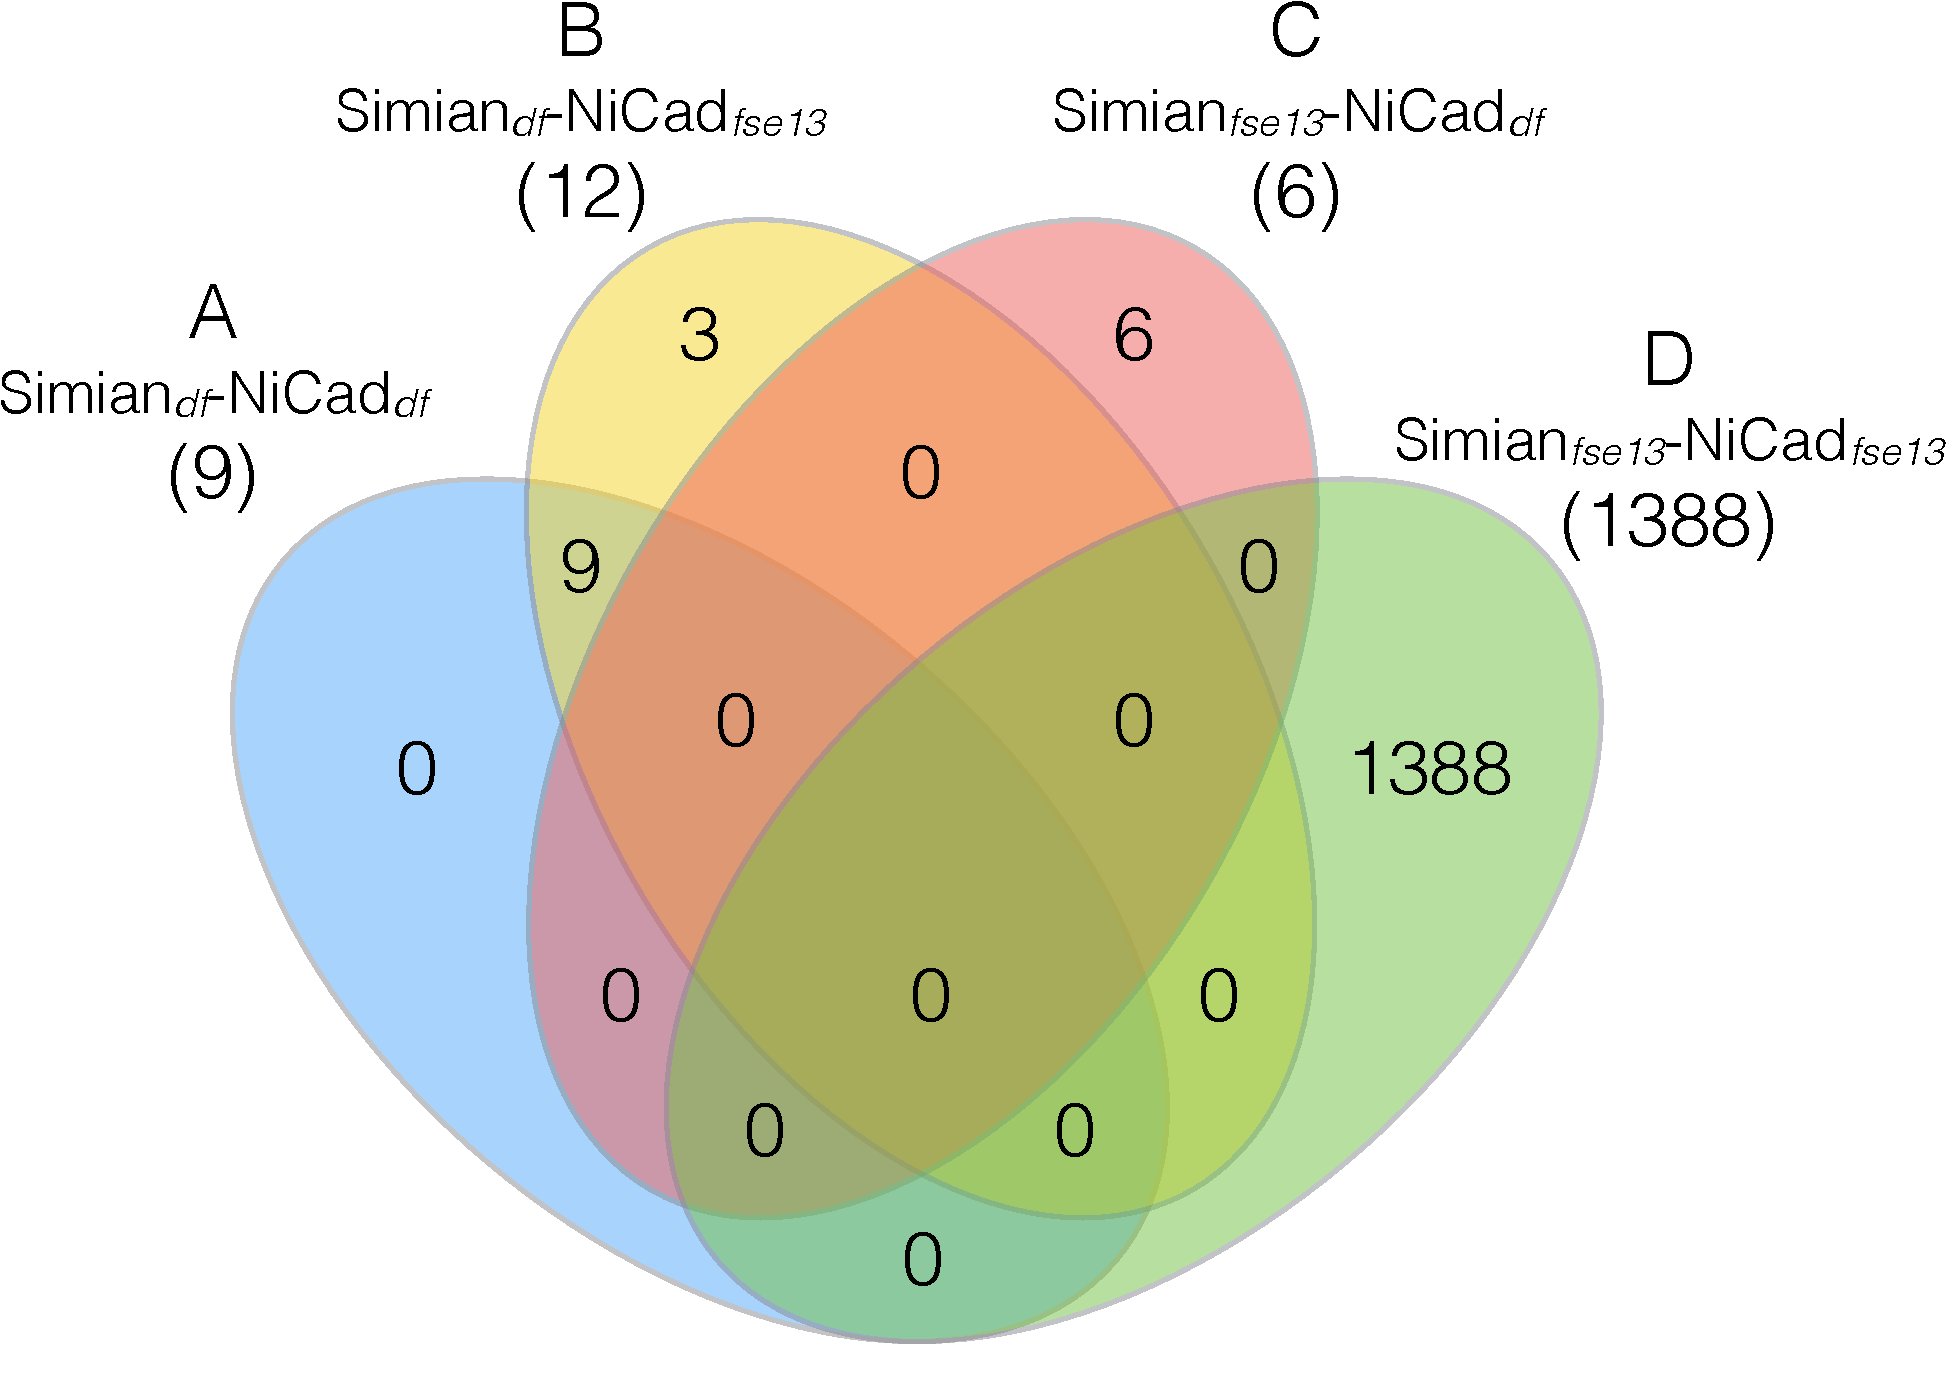
\includegraphics[width=0.7\linewidth]{venn4_pairs_good}
		\captionof{figure}{Qualitas-\textit{O} \textit{good}-match(0.7) pairs}
		\label{fig:venn4_orig_good}
	\end{minipage}%
	\begin{minipage}{.5\textwidth}
		\centering
		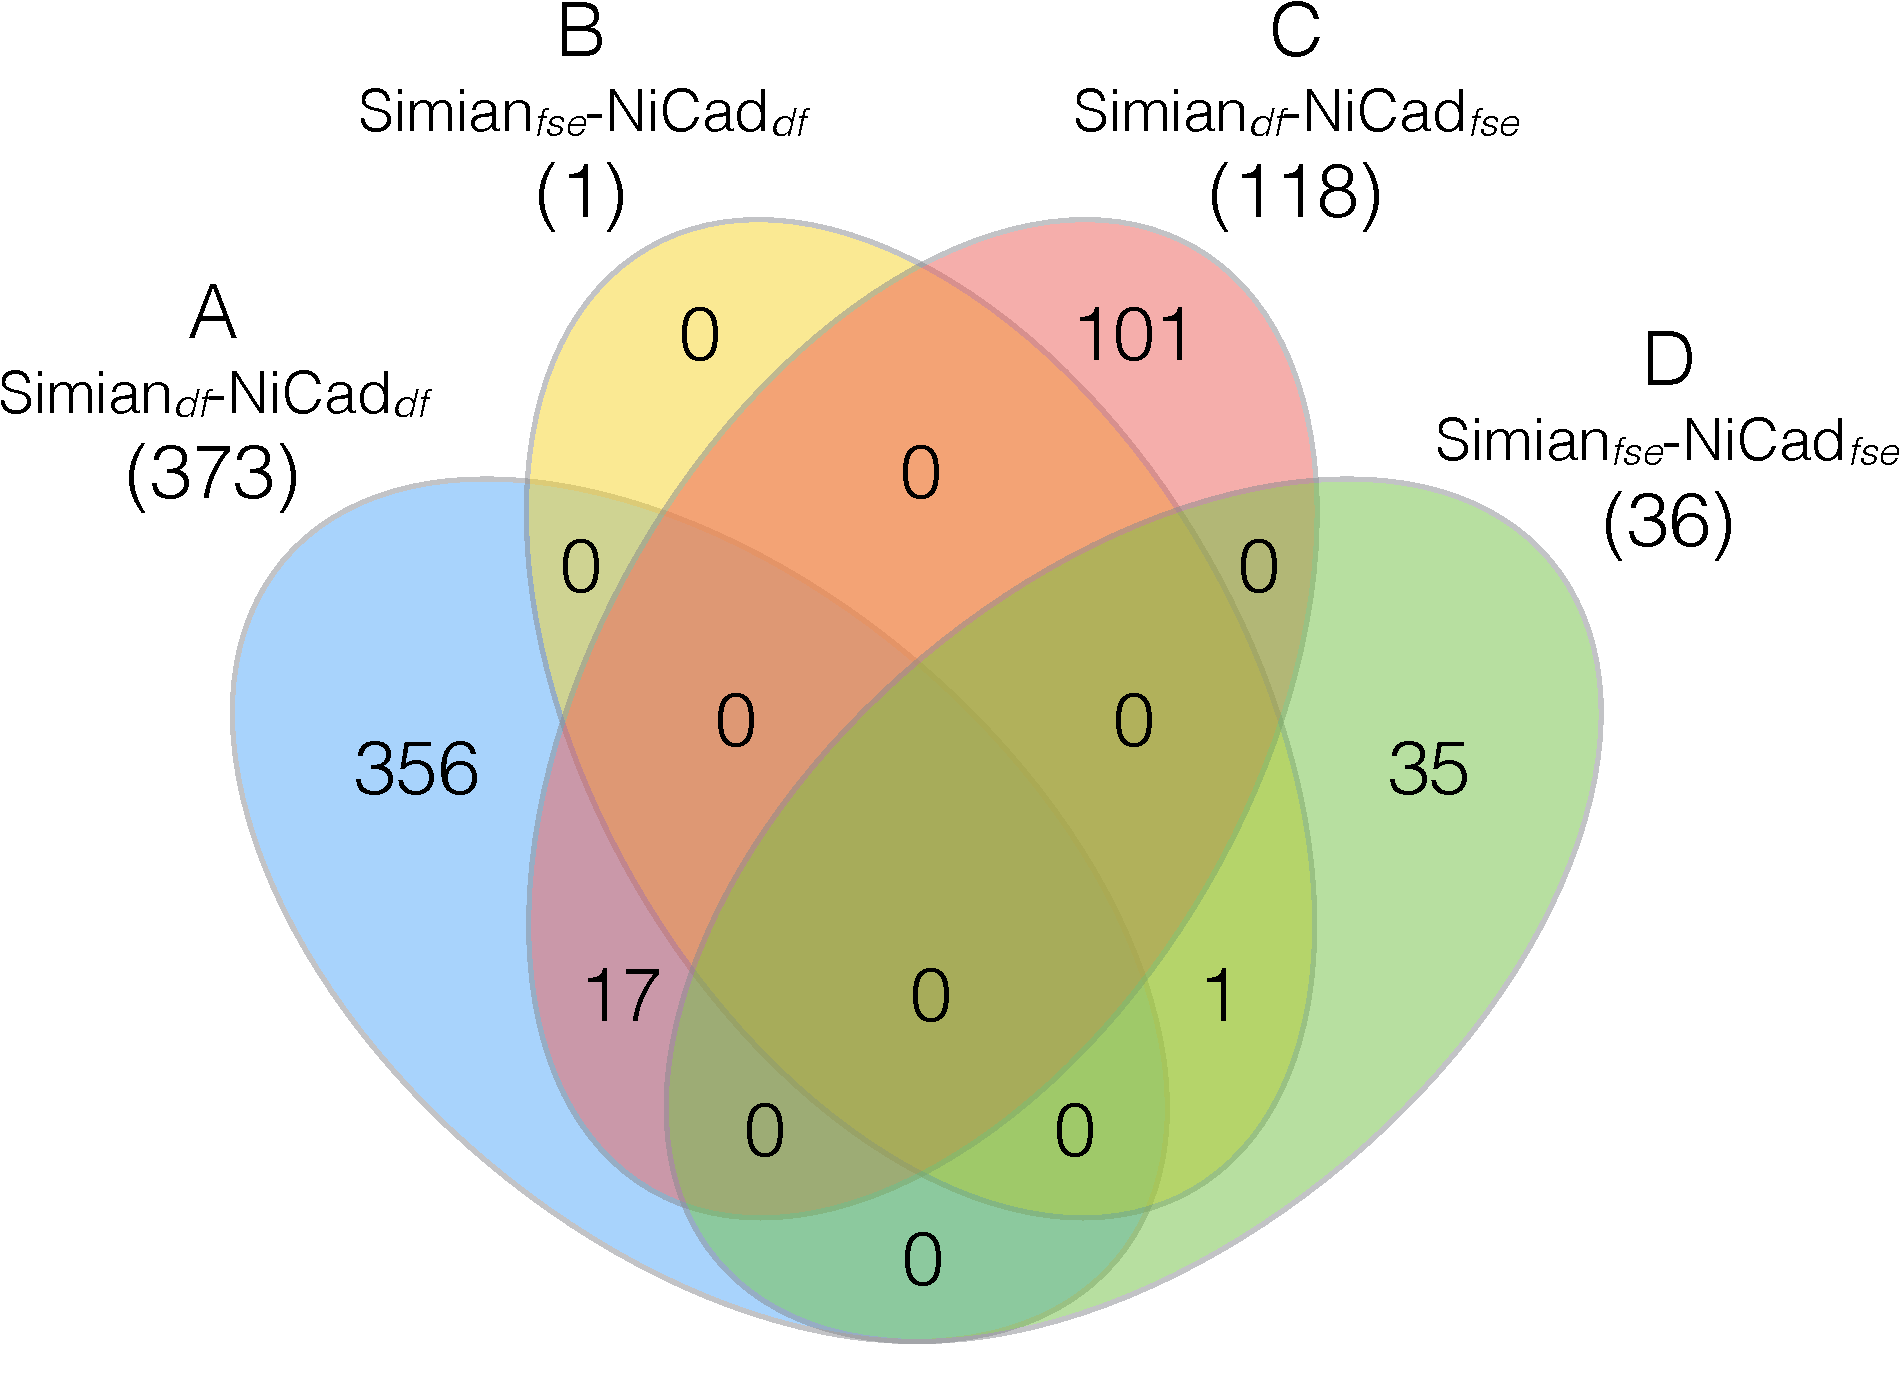
\includegraphics[width=0.7\linewidth]{venn4_pairs_ok}
		\captionof{figure}{Qualitas-\textit{O} \textit{ok}-match(0.7) pairs}
		\label{fig:venn4_orig_ok}
	\end{minipage}
\end{figure}

\begin{figure}
	\centering
	\begin{minipage}{.5\textwidth}
		\centering
		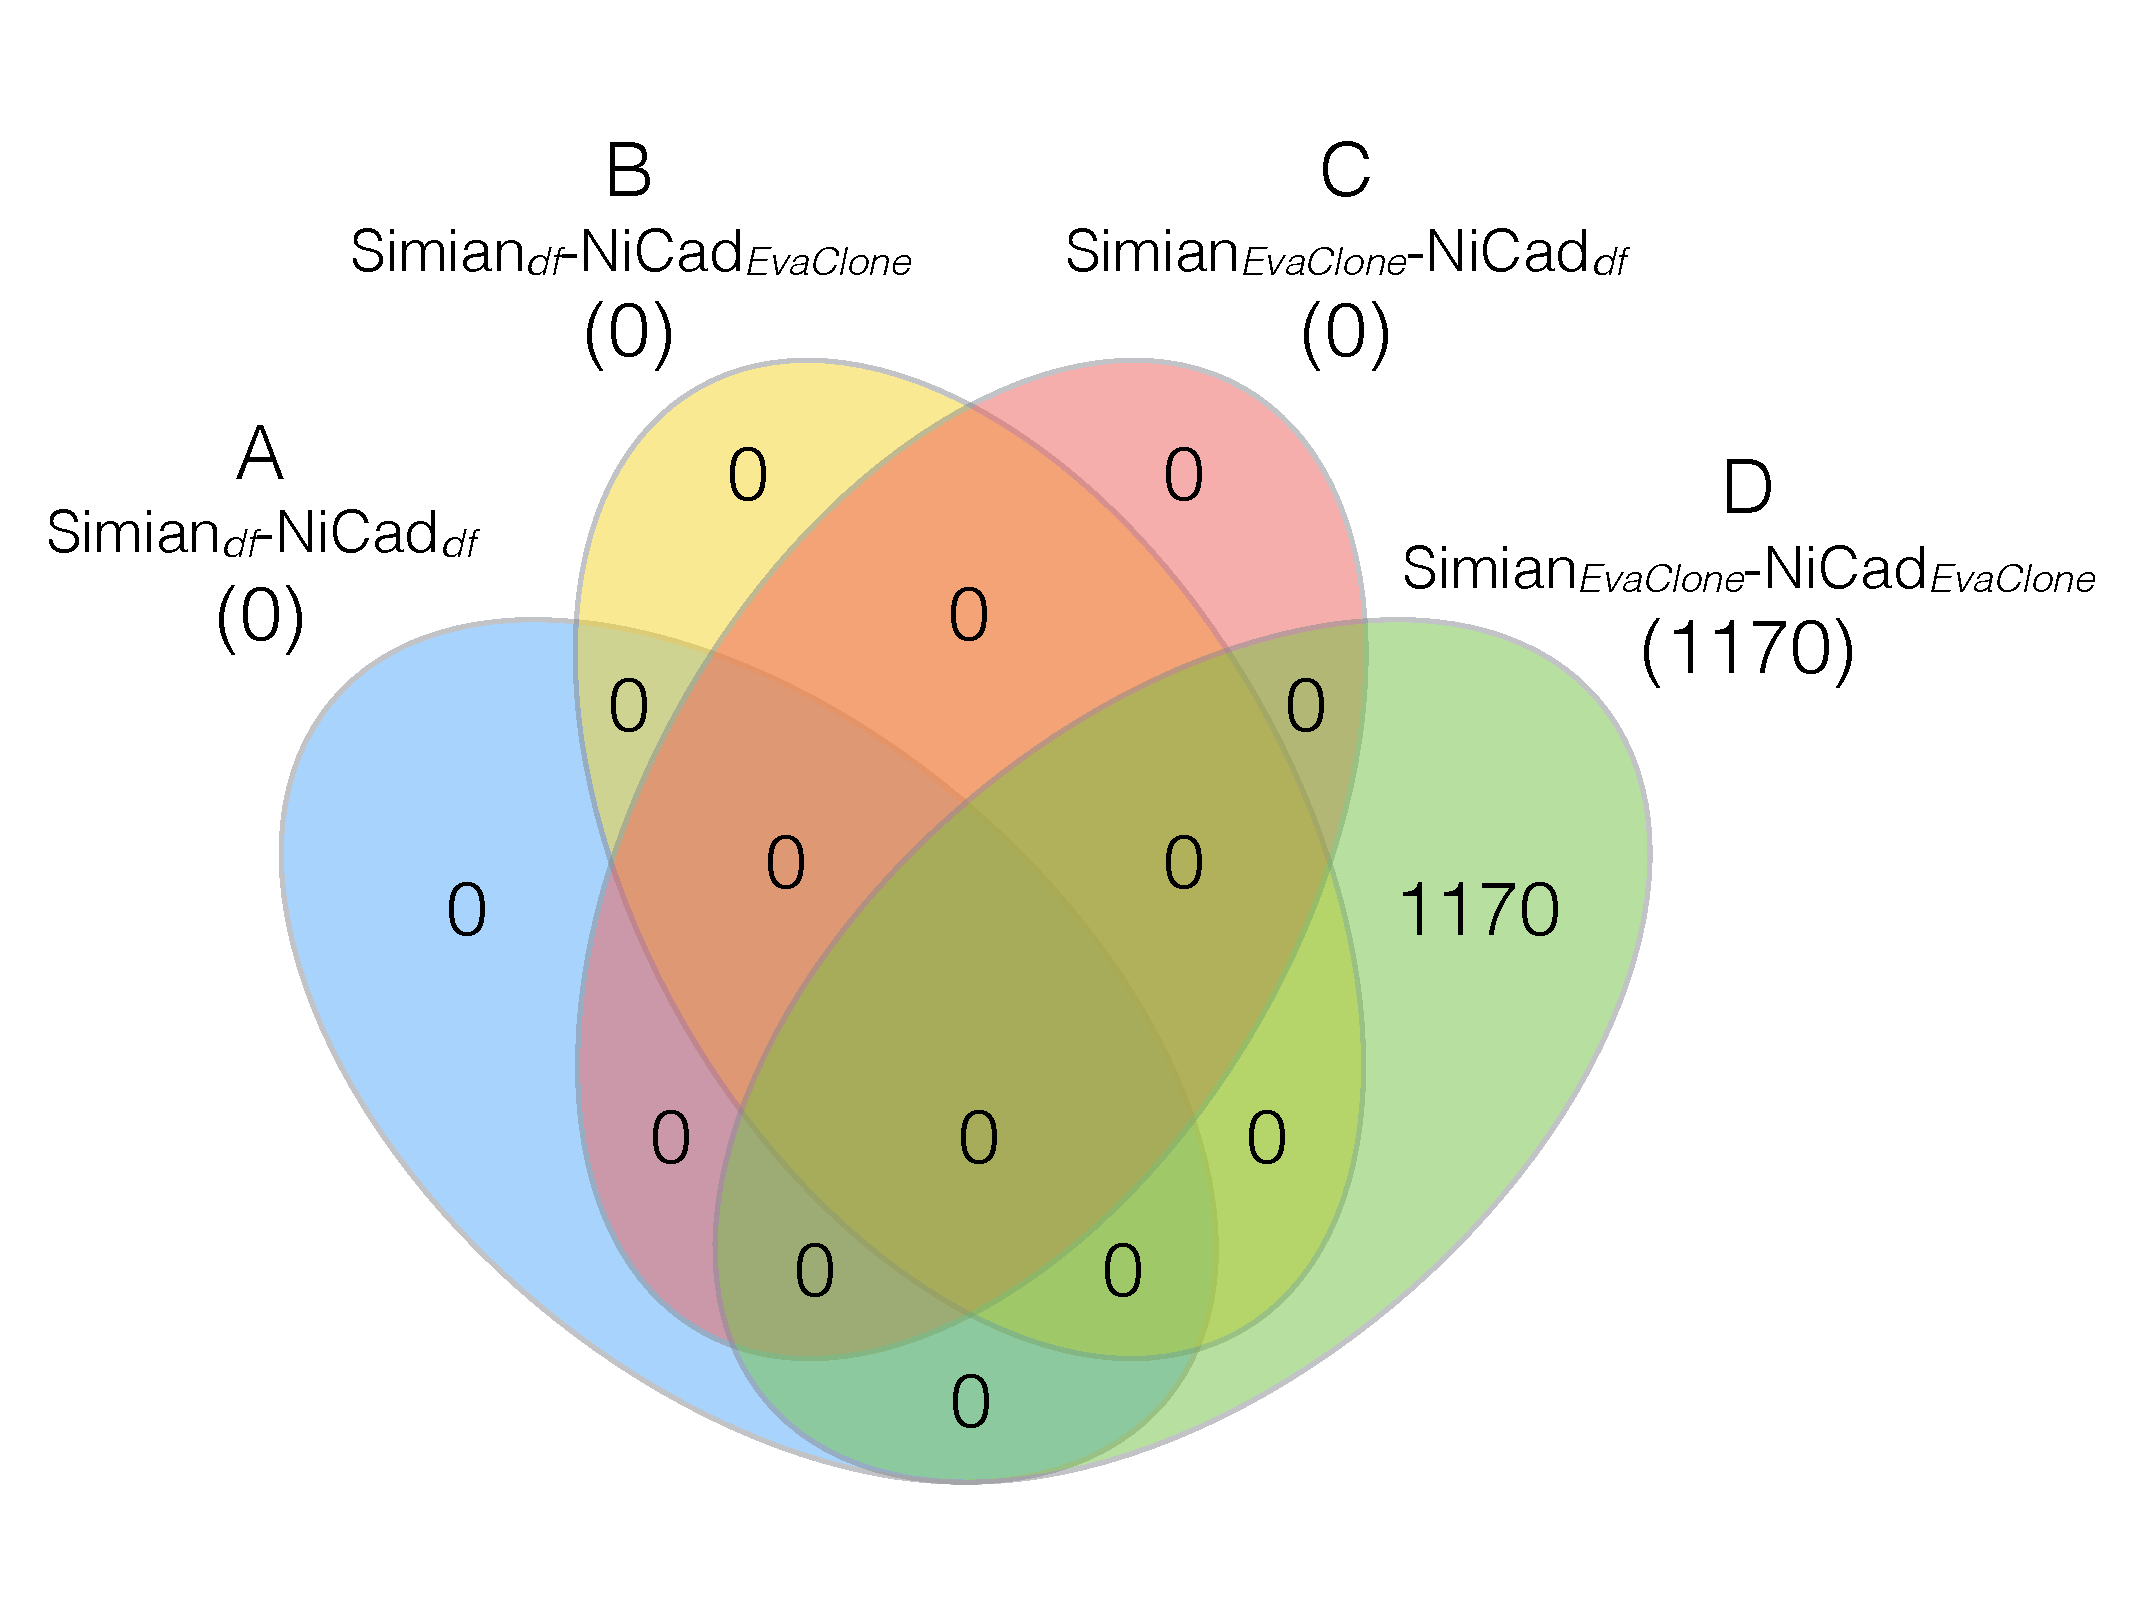
\includegraphics[width=0.7\linewidth]{venn4_pairs_good_new}
		\captionof{figure}{Qualitas-\textit{N} \textit{good}-match(0.7) pairs}
		\label{fig:venn4_new_good}
	\end{minipage}%
	\begin{minipage}{.5\textwidth}
		\centering
		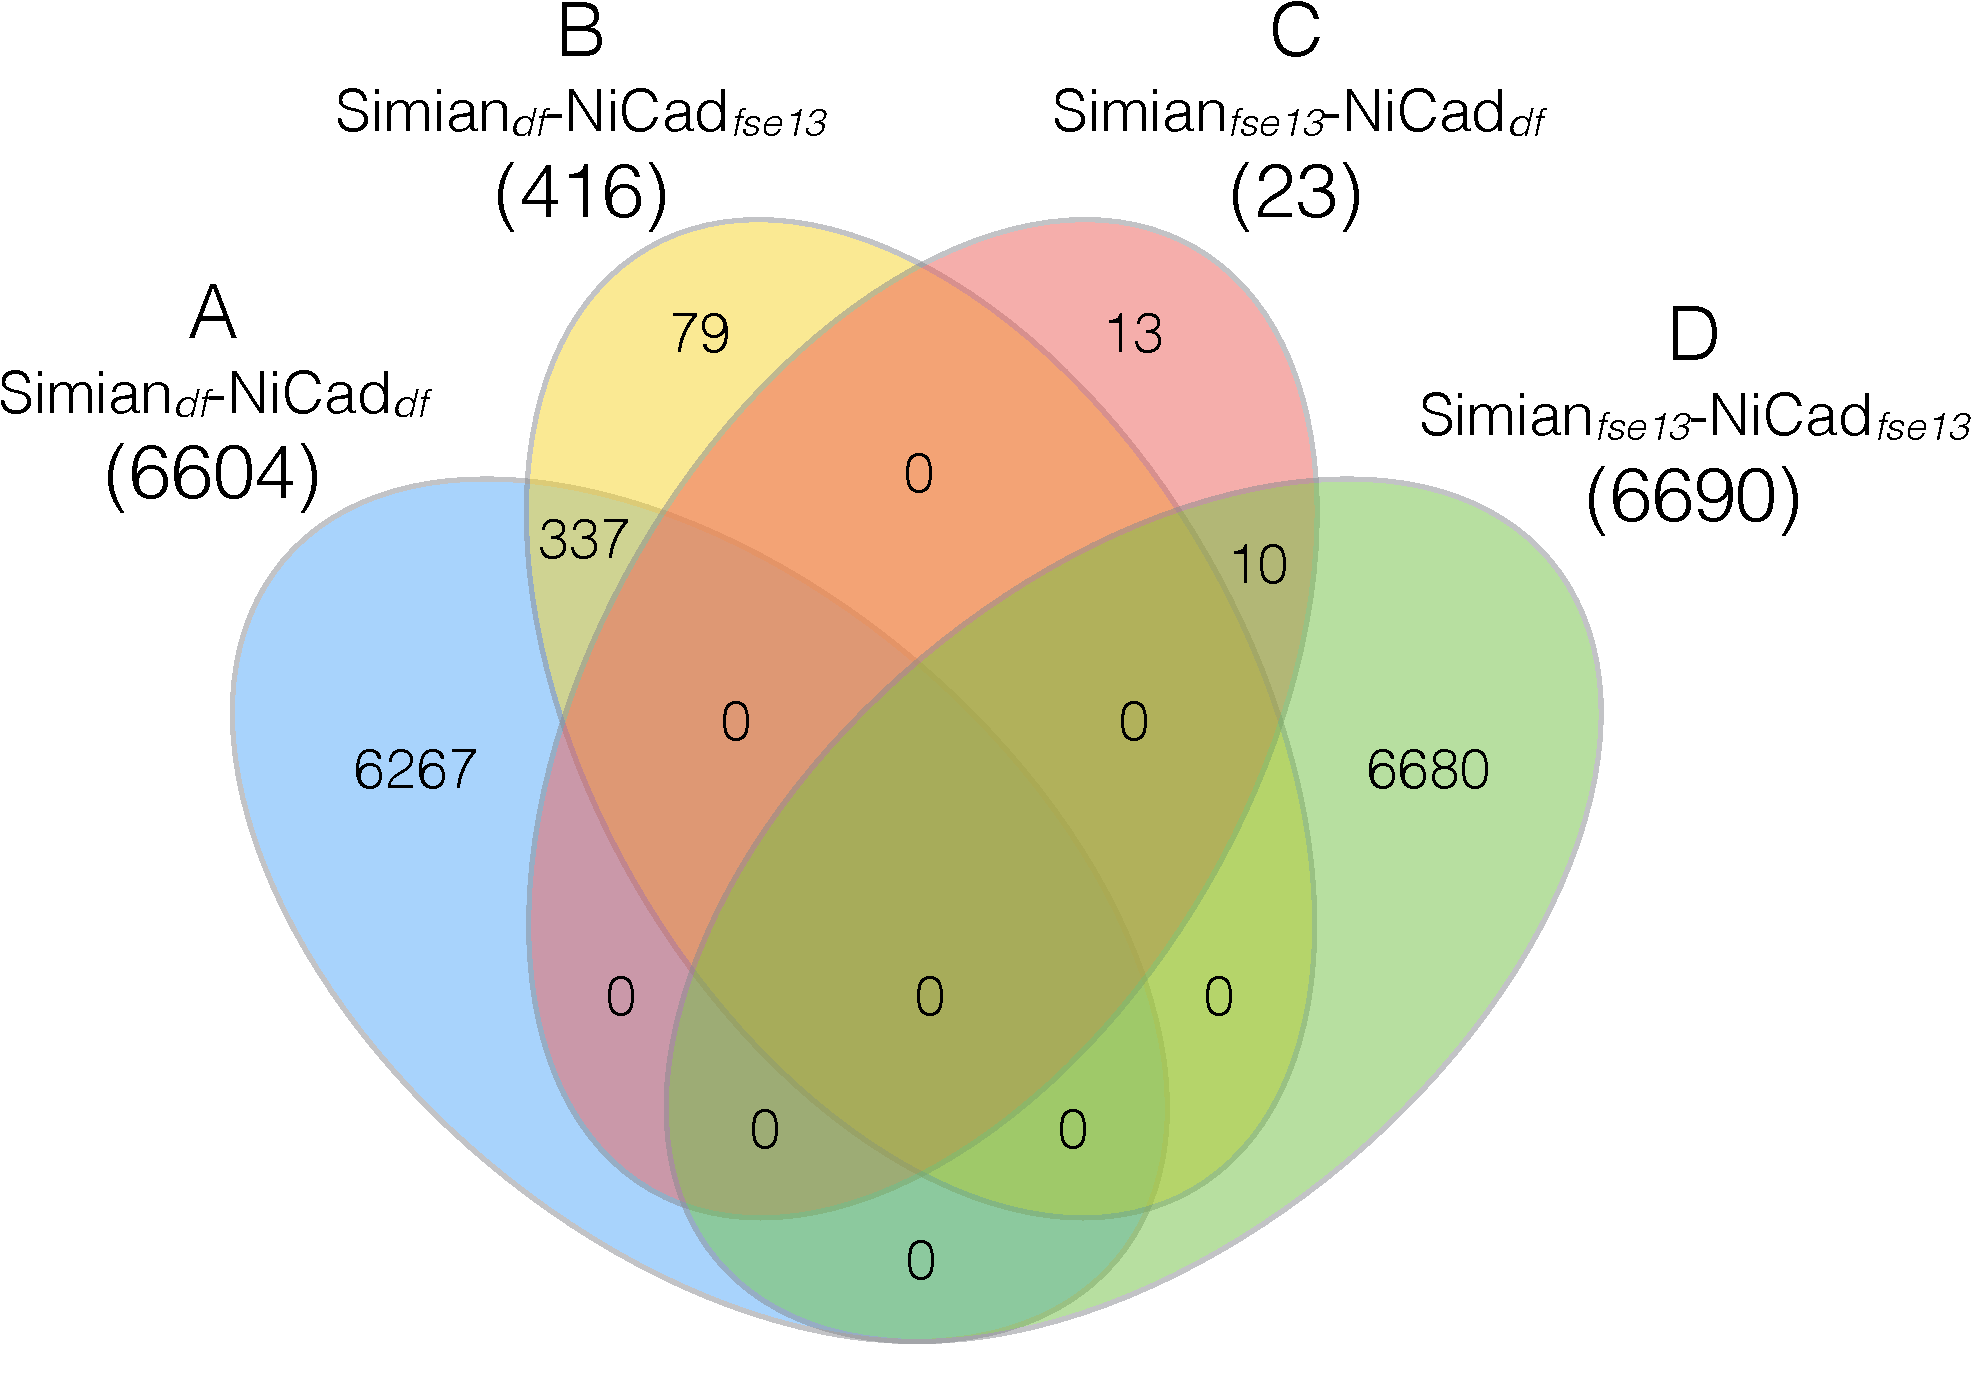
\includegraphics[width=0.7\linewidth]{venn4_pairs_ok_new}
		\captionof{figure}{Qualitas-\textit{N} \textit{ok}-match(0.7) pairs}
		\label{fig:venn4_new_ok}
	\end{minipage}
\end{figure}

\section*{Manual Investigation}

\subsection{Investigation of agreed \textit{good} and \textit{ok}-match clone pairs}

\subsubsection{Qualitas-\textit{O} (v. 2013-09-01r)}

\begin{table}[H]
	\centering
	\caption{Classifications of clone creation}
	\label{tab:classification_scheme}
	\begin{tabular}{|c|p{13cm}|}
		\hline 
		Category & Descriptions \\ 
		\hline 
		A & Code in Stackoverflow is copied from Qualitas (Q $\rightarrow$ S). \\ 
		\hline 
		A' & Code in Qualitas is copied from Stackoverflow (S $\rightarrow$ Q). \\ 
		\hline 
		B & Code is copied either from each other or a third source (unknown) (S $\leftrightarrow$ Q $\vee$ (T $\rightarrow$ S $\wedge$ T $\rightarrow$ Q)).
		\\ 
		\hline 
		C & Code in both places are copied from a third source T (known) (T $\rightarrow$ S $\wedge$ T $\rightarrow$ Q).
		\\ 
		\hline 
		D & Code is a boiler-plate or IDE auto-generated.
		\\ 
		\hline 
		E & Code in both places initialise a similar/the same object; extend the same class/its subclass; implement the same interface.
		\\ 
		\hline 
		F & Accidental similarity, false clone \\ 
		\hline 
	\end{tabular} 
\end{table}

The classification scheme is described in Table \ref{tab:classification_scheme} and the classification results are shown in Table \ref{tab:classification_good_o}. We have manually investigated all of the 1,357 \textit{good-match} ones reported by agreement of four different Simian and NiCad settings.  However, for the \textit{ok-match}, we could not investigate all of the 10,139 pairs manually.  According to the distribution of category from \textit{good-match} results, we can see that Simian$_{\textrm{\textit{fse13}}}$--NiCad$_{\textrm{\textit{fse13}}}$ produces a large number, 1,338, of false positive results (D, E, and F). Thus, we decided to leave them out of the manual investigation of \textit{ok-match} pairs. There are totally 608 \textit{ok-match} pairs that were investigated. The 39 true positive pairs found are combinations of 8 unique Stackoverflow fragments, and 9 unique Qualitas Java files from 6 different projects.

Since we are not certain about the direction of copying in the B-classified pairs, we checked the modification time of each Java file in Qualitas project and compare it to the timestamp of Stackoverflow answers. We found that all Stackoverflow code fragments were posted after their respectively similar Java files in Qualitas project. This means that the copying can only be either (1) Q $\rightarrow$ S or (2) from a third source to both S and Q independently.

\textbf{Qualitas-\textbf{N}:} We decided to filter out the agreed clone pairs reported by agreement of Simian$_{\mathrm{\textit{fse13}}}$-NiCad$_{\mathrm{\textit{fse13}}}$ altogether due to its large number of false positive. With the remaining 3 agreements, we did manual investigation of agreed \textit{ok}-match clone pairs from agreements of Simian$_{\mathrm{\textit{df}}}$-NiCad$_{\mathrm{\textit{df}}}$, Simian$_{\mathrm{\textit{df}}}$-NiCad$_{\mathrm{\textit{fse13}}}$, and Simian$_{\mathrm{\textit{fse13}}}$-NiCad$_{\mathrm{\textit{df}}}$. We had not done any investigation of \textit{good}-match since there were no \textit{good}-match pairs for these 3 agreements. The number of pairs that have been looked at is 6,706 (excluding duplicates). The results are shown in Table.

\begin{table}[H]
	\centering
	\caption{Qualitas-\textit{O}: Classification results of \textit{good-} and \textit{ok}-match pairs which excludes the subsumed \textit{good}-match and Simian$_{\mathrm{\textit{fse13}}}$-NiCad$_{\mathrm{\textit{fse13}}}$ pairs.}
	\label{tab:classification_good_o}
	\begin{tabular}{|l"r|r|r|r|r|r|r|r"r|r|r|r|r|r|r"r|r|r|r|}
		\hline
		Classificaiton & A & A' & B & C & \textbf{Sum} & S$_{u}$ & Q$_u$ & Q$_{up}$ & D  & E & F & \textbf{Sum} & S$_{u}$ & Q$_u$ & Q$_{up}$ & \textbf{Total}  & S$_{u}$ & Q$_u$ & Q$_{up}$\\ 
		\hline 
		\multirow{1}{*}{\textit{good-match(0.7)}}  & 1 & 0 & 1  & 3 & \textbf{5} & 5 & 4 & 4 & 26  & 6 & 1320 & \textbf{1352} & 56 & 402 & 31 & \textbf{1357} & 61 & 406 & 32 \\
		\multirow{1}{*}{\textit{ok-match(0.7)}}  & 8 & 0 & 23  & 8 & \textbf{39} & 8 & 9 & 6 & 480 & 28 & 61 & \textbf{569} & 76 & 60 & 16 & \textbf{608} & 83 & 68 & 19 \\
		\hline
	\end{tabular} 
\end{table}

%\begin{table}[H]
%	\centering
%	\caption{Classification results of \textit{good-} and \textit{ok}-matches (excluding the subsumed \textit{good}-match pairs).}
%	\label{tab:classification}
%	\begin{tabular}{|l|R{3mm}|R{3mm}|R{3mm}|R{3mm}|R{5mm}|R{3mm}|R{7mm}|R{7mm}|R{3mm}|R{3mm}|R{3mm}|R{3mm}|R{7mm}|R{3mm}|R{7mm}|R{7mm}|}
%		\hline
%		\multirow{2}{*}{Classification}	& \multicolumn{8}{c|}{Qualitas-\textit{O}} & \multicolumn{8}{c|}{Qualitas-\textit{N}} \\ 	\cline{2-17}
%		 & A & A' & B & C & D & E & F & Total 
%		 & A & A' & B & C & D & E & F & Total \\ 
%		\hline 
%		\multirow{1}{*}{\textit{good-match(0.7)}} 
%		& 1 & 0 & 1  & 3 & 26  & 6 & 1,369 & 1,406 
%		& -- & -- & -- & -- & -- & -- & -- & --  \\ \cline{2-8}
%		\hline
%		\multirow{1}{*}{\textit{ok-match(0.7)}} 
%		& 8  & 0 & 36 & 8 & 474 & 57 & 81 & 664 
%		& 2 & 0 & 0 & 0 & 6,676 & 1 & 27 & 6,706 \\ \cline{2-8}
%		\hline
%		TP/FP
%		& \multicolumn{4}{c|}{57} & \multicolumn{3}{c|}{2,013} & 2,070
%		& \multicolumn{4}{c|}{2} & \multicolumn{3}{c|}{6,704} & 6,706 \\ 
%		\hline
%		Unique SO fragments & \multicolumn{4}{c|}{10} & & & & & \multicolumn{4}{c|}{1} & & & & \\
%		\hline
%		Unique Q files & \multicolumn{4}{c|}{13} & & & & & \multicolumn{4}{c|}{1} & & & & \\
%		\hline
%		Unique Q projects & \multicolumn{4}{c|}{8} & & & & & \multicolumn{4}{c|}{1} & & & & \\
%		\hline
%	\end{tabular} 
%\end{table}

\begin{table}[H]
	\centering
	\caption{Qualitas-\textit{O}: Distribution of classification category A--F according to \textit{good}-match pairs}
	\label{tab:good_classification}
	\begin{tabular}{|l|r|r|r|r|r|r|r|r|}
		\hline 
		Category   & A   & 	A'   & 	B   & C   & D   &	E   &	F   & Total  \\
		\hline
		Simian$_{\mathrm{\textit{df}}}$--NiCad$_{\mathrm{\textit{df}}}$   & 1 & 0 & 1 & 3 & 0 & 4 & 0 & 9 \\
		Simian$_{\mathrm{\textit{df}}}$--NiCad$_{\textrm{\textit{fse13}}}$   & 1 & 0 & 1 & 3 & 1 & 5 & 1 & 12 \\
		Simian$_{\textrm{\textit{fse13}}}$--NiCad$_{\mathrm{\textit{df}}}$   & 0 & 0 & 0 & 0 & 7 & 0 & 0 & 7 \\
		Simian$_{\textrm{\textit{fse13}}}$--NiCad$_{\textrm{\textit{fse13}}}$   & 0 & 0 & 0 & 0 & 18 & 1 & 1,319 & 1,338 \\
		\hline
		Total   &   2   &   0   &  2   &  6   &   26   &   10   & 1,320  & 1,366 \\
		Total (unique)  &   1   &   0   &  1   &  3   &   26   &   6   & 1,320  & 1,352 \\
		\hline
	\end{tabular} 
\end{table}

\begin{table}[H]
	\centering
	\caption{Qualitas-\textit{O}: Distribution of classification category A--F  according to the \textit{ok}-match pairs}
	\label{tab:ok_classification}
	\begin{tabular}{|l|r|r|r|r|r|r|r|r|}
		\hline 
		Category   																										& A   	& 	A' 	& 	B  & C	   & D   	&	E   &	F   & Total  \\
		\hline
		Simian$_{\mathrm{\textit{df}}}$--NiCad$_{\mathrm{\textit{df}}}$        & 3 	& 0 	& 10	& 6 	& 433  & 5	& 7  &  464 \\
		Simian$_{\mathrm{\textit{df}}}$--NiCad$_{\textrm{\textit{fse13}}}$   									& 8 	& 0 	& 22	& 4	& 250 & 25  & 32 &  341 \\
		Simian$_{\textrm{\textit{fse13}}}$--NiCad$_{\mathrm{\textit{df}}}$   									& 0 	& 0 	& 0 	& 0 	 & 29 	  & 0 		& 24 	& 53 \\
		\hline
		Total   &   11  &   0   &  32   &  10   &   712   &   30   & 63  & 858 \\
		Total (unique)  &   8  &   0   &  23   &  8   &  480  &  28  & 61  & 608 \\
		\hline
	\end{tabular} 
\end{table}

\subsubsection{Qualitas-\textit{N} (v. 2016-08-05)}
We decided to filter out the agreed clone pairs reported by agreement of Simian$_{\mathrm{\textit{fse13}}}$-NiCad$_{\mathrm{\textit{fse13}}}$ altogether due to its large number of false positive. With the remaining 3 agreements, we did manual investigation of agreed \textit{ok}-match clone pairs from agreements of Simian$_{\mathrm{\textit{df}}}$-NiCad$_{\mathrm{\textit{df}}}$, Simian$_{\mathrm{\textit{df}}}$-NiCad$_{\mathrm{\textit{fse13}}}$, and Simian$_{\mathrm{\textit{fse13}}}$-NiCad$_{\mathrm{\textit{df}}}$. We had not done any investigation of \textit{good}-match since there were no \textit{good}-match pairs for these 3 agreements. The number of pairs that have been looked at is 6,706 (excluding duplicates). The results are shown in Table \ref{tab:classification_good_n}.

\begin{table}[H]
	\centering
	\caption{Qualitas-\textit{N}: Classification results of \textit{good-} and \textit{ok}-matches (excluding the subsumed \textit{good}-match pairs).}
	\label{tab:classification_good_n}
	\begin{tabular}{|l"r|r|r|r|r|r|r|r"r|r|r|r|r|r|r"r|r|r|r|}
		\hline
		Classificaiton & A & A' & B & C & Sum & S$_{u}$ & Q$_u$ & Q$_{up}$ & D  & E & F & Sum & S$_{u}$ & Q$_u$ & Q$_{up}$ & Total  & S$_{u}$ & Q$_u$ & Q$_{up}$\\ 
		\hline 
		\multirow{1}{*}{\textit{good-match(0.7)}}  & - & - & - & - & - & - & - & - & - & - & - & - & - & - & - & - & - & - & - \\
		\multirow{1}{*}{\textit{ok-match(0.7)}}  & 2 & 0 & 0 & 0 & & & & & 6676 & 1 & 27 & & & & & 6706 & & & \\
		\hline
	\end{tabular} 
\end{table}

%\begin{table}[H]
%	\centering
%	\caption{Classification results of 6,706 \textit{ok}-matches of Simian$_{\mathrm{\textit{df}}}$-NiCad$_{\mathrm{\textit{df}}}$, Simian$_{\mathrm{\textit{df}}}$-NiCad$_{\mathrm{\textit{fse13}}}$.}
%	\label{tab:classification_new}
%	\begin{tabular}{|l|r|r|r|r|r|r|r|r|}
%		\hline 
%		Classification & A & A' & B & C & D & E & F & Total \\ 
%		\hline
%		\multirow{1}{*}{\textit{good-match(0.7)}} & -- & -- & -- & -- & -- & -- & -- & -- \\ \cline{2-8}
%		\hline
%		\multirow{1}{*}{\textit{ok-match(0.7)}}  \\ \cline{2-8}
%		\hline
%		\multirow{3}{*}{TP/FP} & \multicolumn{4}{c|}{2} & \multicolumn{3}{c|}{\multirow{3}{*}{6704}} & \multirow{3}{*}{6706} \\ 
%		& \multicolumn{4}{l|}{\textit{1 unique SO fragments}} & \multicolumn{3}{c|}{} & \\
%		& \multicolumn{4}{l|}{\textit{1 unique Q files}} & \multicolumn{3}{c|}{} & \\
%		\hline
%	\end{tabular} 
%\end{table}

\begin{table}[H]
	\centering
	\caption{Qualitas-\textit{N}: Distribution of classification category A--F  according to the \textit{ok}-match pairs}
	\label{tab:ok_classification_new}
	\begin{tabular}{|l|r|r|r|r|r|r|r|r|}
		\hline 
		Category   																										& A   	& 	A' 	& 	B  & C	   & D   	&	E   &	F   & Total  \\
		\hline
		Simian$_{\mathrm{\textit{df}}}$--NiCad$_{\mathrm{\textit{df}}}$ & 0 & 0	& 0 & 0 & 6603 & 1 & 0 & 6604 \\
		Simian$_{\mathrm{\textit{df}}}$--NiCad$_{\textrm{\textit{fse13}}}$ 
		& 2 	& 0 	& 0 	& 0 	& 73 	 & 0 	  & 4 		&  79 \\
		Simian$_{\textrm{\textit{fse13}}}$--NiCad$_{\mathrm{\textit{df}}}$   									
		& 0 	& 0 	& 0 	& 0 	 & 0 	  & 0 		& 23 	& 23 \\
		\hline
		Total   & 2  	&   0   & 0   	&  0   &   6676   &   1   & 27  & 6706 \\
		\hline
	\end{tabular} 
\end{table}

\begin{figure}
	\centering
	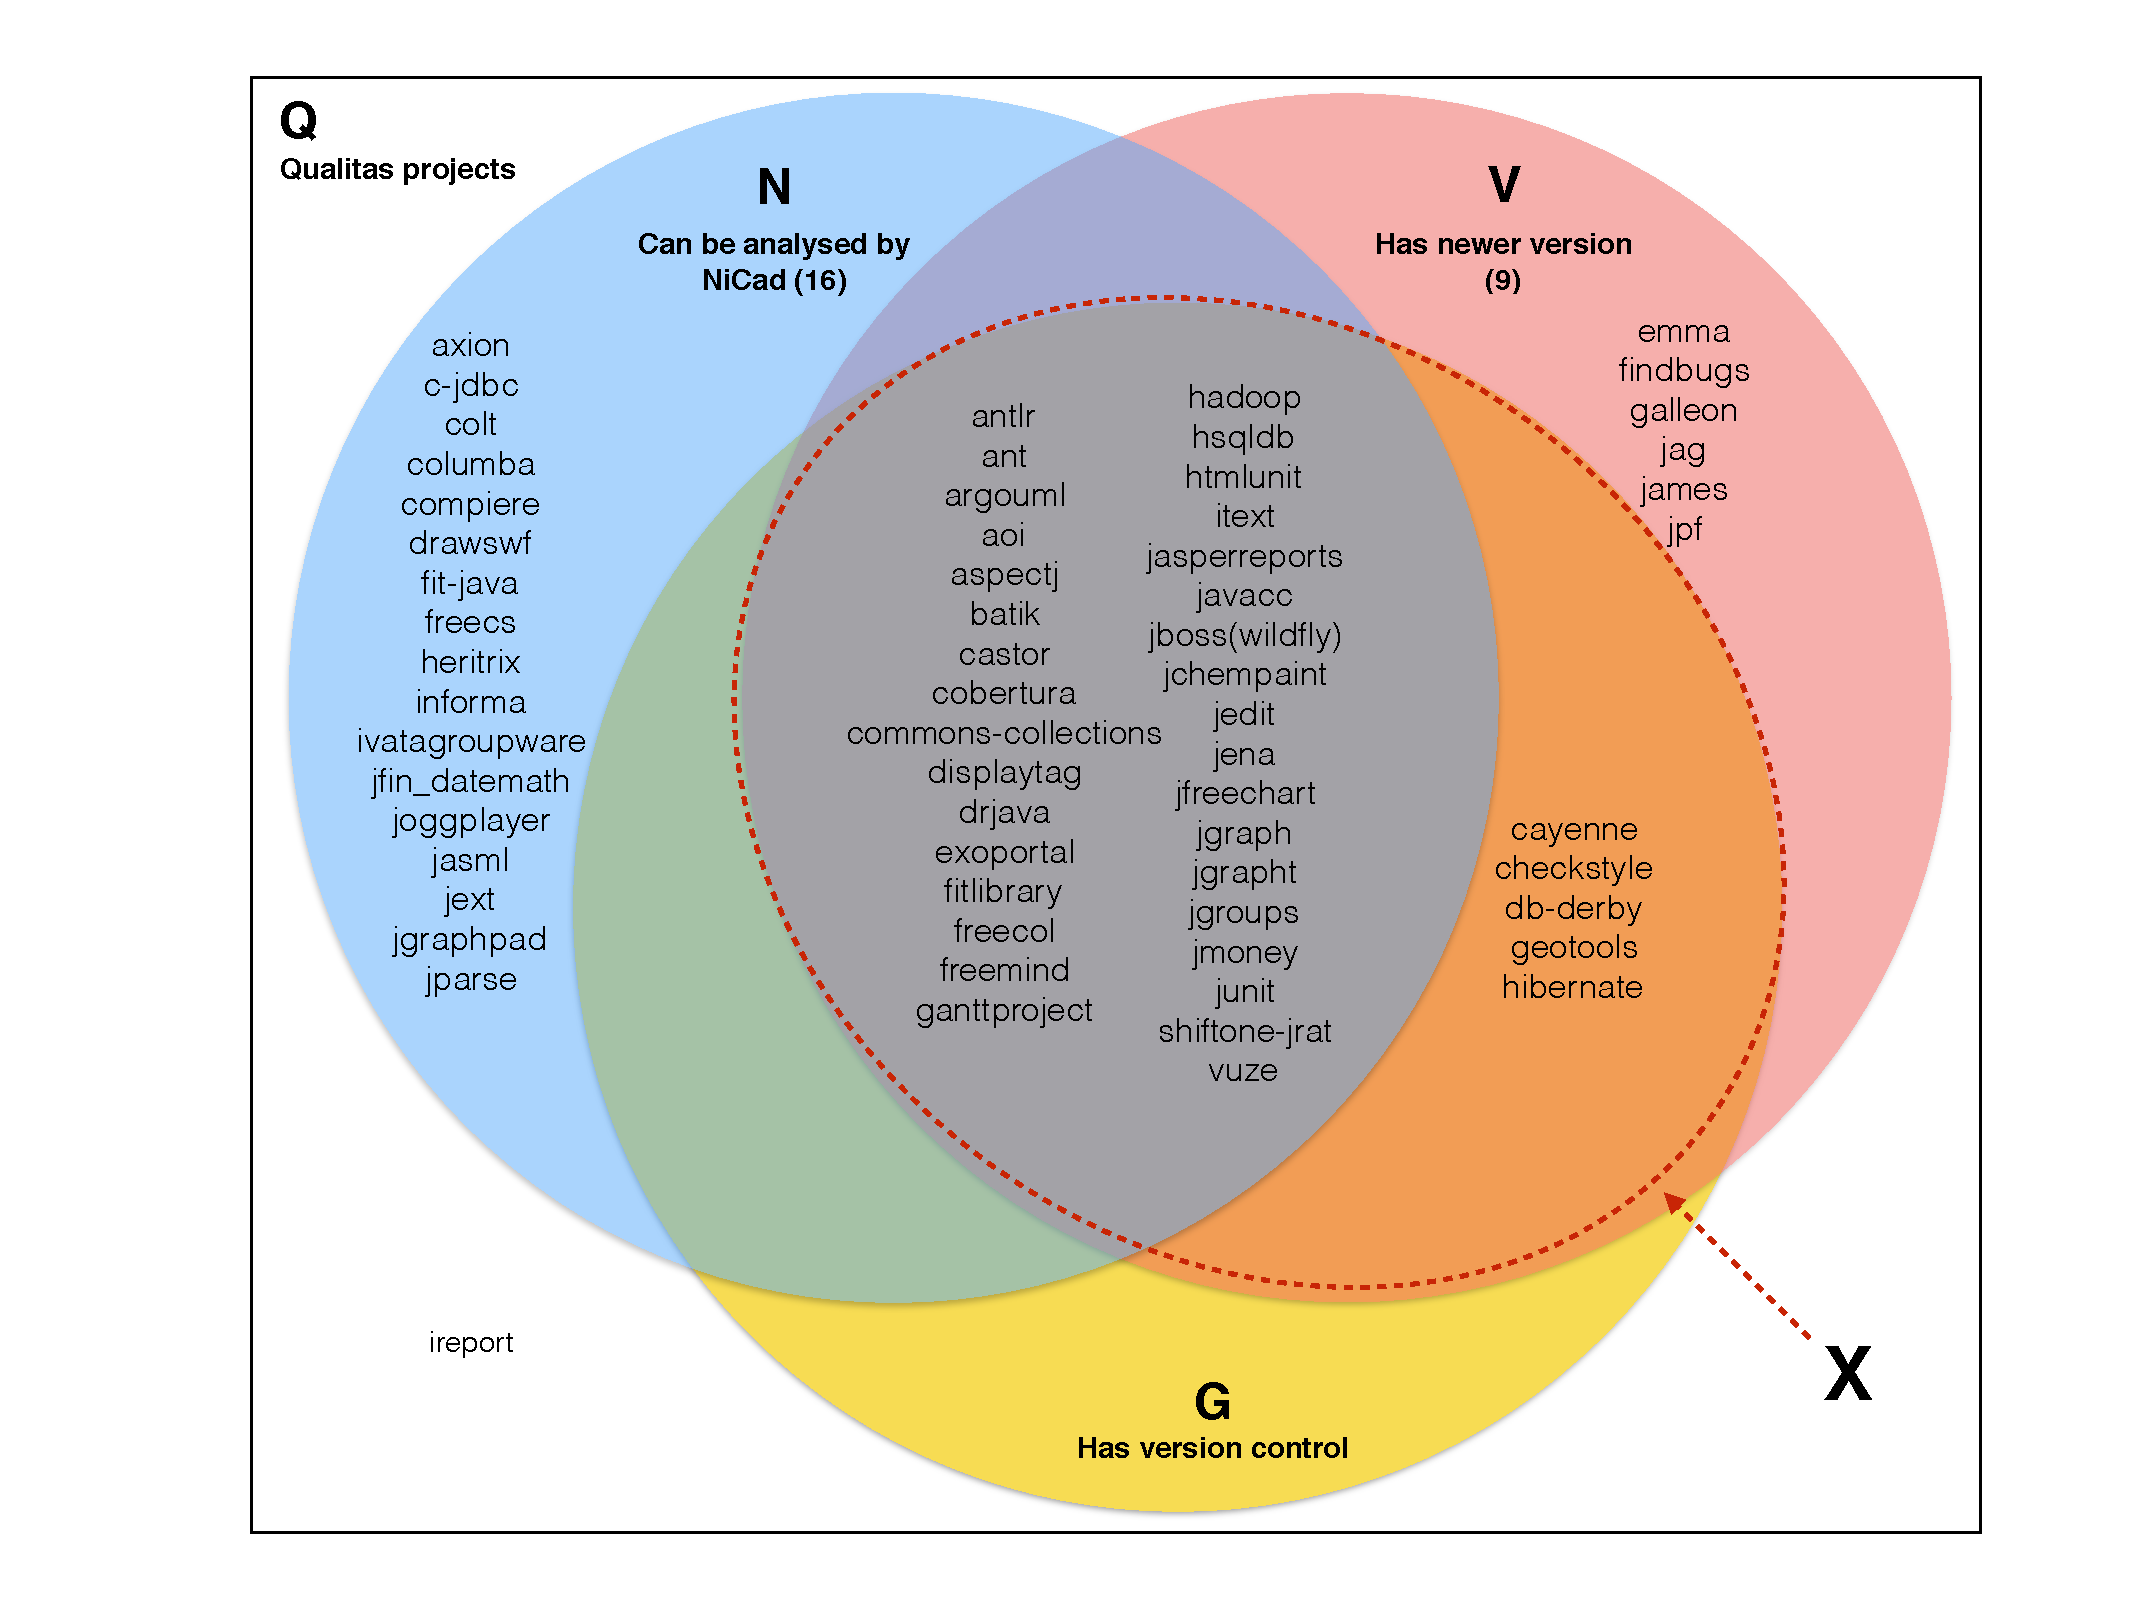
\includegraphics[width=0.7\linewidth]{n+v+g}
	\caption{Qualitas projects categorised by NiCad's results, existence of newer versions, and version control}
	\label{fig:n+v+g}
\end{figure}

\subsection{Investigation of Simian and NiCad clone pairs}
\subsubsection{Qualitas-\textit{O} (v. 2013-09-01r)}
In the preliminary stage of our experiment, we found that there are 41 Stackoverflow fragments reported by Simian with default configurations. However, only 10 of them appear in the new results using tool's agreement. Thus, we further investigated the clone pairs reported by Simian and NiCad but \textit{without} an agreement. 

With our 4 settings, we decided to investigate only 2 settings, Simian$_{\mathrm{\textit{df}}}$, and NiCad$_{\mathrm{\textit{df}}}$, and drop Simian$_{\mathrm{\textit{fse13}}}$ and NiCad$_{\mathrm{\textit{fse13}}}$ due to their large number of false positives as shown in Table \ref{tab:good_classification} and \ref{tab:ok_classification}. With the 2 selected settings, we investigated clone pairs having the minimum clone size of 10 SLOC as they are meaningful and tend to be real clone in modern clone detection \cite{Sajnani2016}. 

For Simian$_{\mathrm{\textit{df}}}$, there were 9,393 clone pairs reported by the tool. Out of 9,393 pairs, 143 of them are the ones found in \textit{ok-}pairs using agreement-based detection. We filtered the results further by removing false positives such as similar equals(), hashCode() methods, getters and setters out by using regular expression. We managed to remove 8,958 pairs using this method. Eventually, there were 292 clone pairs remaining for manual investigation. For NiCad$_{\mathrm{\textit{df}}}$, we obtained 7,062 clone pairs to look at which is infeasible for manual investigation. Hence, result filtering was also needed. However, regular expressions could not be used effectively as in Simian's case since NiCad allowed clones that are different at keywords/variable names or even added/deleted lines. So we decided to filter the results by selecting pairs that pass stricter clone criteria with $\mathrm{UPI} = 0.2$. By reducing the UPI to 0.2, there were totally 171 pairs left. Out of 171, 57 are \textit{ok}-pairs and 114 are remaining pairs for manual check (18 pairs are from \textit{cayenne} and \textit{iReport} that could not be analysed using UPI = 0.3). The statistics of the clones and classification results are reported in Table \ref{tab:classification_indv_stats} and \ref{tab:classification_indv}.

%We selected only Stackoverflow fragment and Qualitas files that have never been looked at before in the previous investigation. If many clone pairs having the same Stackoverflow fragment and Qualitas file, we keep only the largest one. The reason for having this criteria is that we found a lot of duplicate clone pairs with the same classifications from either Stackoverflow fragments or Qualitas files. The classification results are shown in Table \ref{tab:classification_indv}. 

\begin{table}[H]
	\centering
	\caption{Statistics of Simian$_{\mathrm{\textit{df}}}$ and NiCad$_{\mathrm{\textit{df}}}$ clone pairs.}
	\label{tab:classification_indv_stats}
	\begin{tabular}{l|r|r|r|r}
		\hline 
		Tool & Clone pairs & \textit{ok}-pairs & filtered pairs & remaining pairs \\ 
		\hline 
		\multirow{1}{*}{\textit{Simian$_{\mathrm{\textit{df}}}$}} & 9393 & 143 & 8958 & 292 \\
		\hline
		\multirow{1}{*}{\textit{NiCad$_{\mathrm{\textit{df}}}$}} & 7062  & 231 & 6717 & 114 \\
		\hline
	\end{tabular} 
\end{table}

\begin{table}[H]
	\centering
	\caption{Classification results of 292 Simian$_{\mathrm{\textit{df}}}$ and 114 NiCad$_{\mathrm{\textit{df}}}$ individual unique pairs. NiCad$_{\mathrm{\textit{df}}}$* shows the classification without cayenne and iReport.}
	\label{tab:classification_indv}
	\begin{tabular}{|l|r|r|r|r|r|r|r|r|r|r|r|r|r|r|r|r|r|r|r|}
		\hline 
		Tool/Classification & A & A' & B & C & \textbf{Sum} & S$_{u}$ & Q$_{u}$ & Q$_{up}$ & D & E & F & \textbf{Sum}  & S$_{u}$ & Q$_{u}$ & Q$_{up}$ & \textbf{Total} & S$_{u}$ & Q$_{u}$  & Q$_{up}$  \\ 
		\hline 
		\multirow{1}{*}{\textit{Simian$_{\mathrm{\textit{df}}}$}} & 35 & 0 & 90 & 8 & \textbf{133} & 68 & 59 & 23 & 13 & 12 & 134 & \textbf{159} & 39 & 72 & 23 & \textbf{292} & 103 & 125 & 31 \\
		\hline
		\multirow{1}{*}{\textit{NiCad$_{\mathrm{\textit{df}}}$}} & 4  & 0 & 5 & 0 & \textbf{9} & 9 & 5 & 4 & 24 & 3 & 78 & \textbf{105} & 41 & 39 & 12 & \textbf{114} & 48 & 44 & 14 \\ 
		\hline
		\multirow{1}{*}{\textit{NiCad$_{\mathrm{\textit{df}}}$}*} & 4  & 0 & 1 & 0 & \textbf{5} & 4 & 5 & 3 & 23 & 1 & 67 & \textbf{91} & 28 & 31 & 10 & \textbf{96} & 33 & 37 & 13 \\ 
		\hline
	\end{tabular} 
\end{table}

\begin{table}[H]
	\centering
	\caption{Numbers of true online clone pairs (A+A'+B+C) found by manual investigation}
	\label{tab:classification_indv_summary}
	\begin{tabular}{r|r|r|r|r}
		\hline 
		\textit{good}-pairs & \textit{ok}-pairs & Simian$_{\mathrm{\textit{df}}}$ pairs & NiCad$_{\mathrm{\textit{df}}}$ pairs & Total \\ 
		\hline 
		5 & 52 & 133 & 9 & 183 \\
		\hline
	\end{tabular} 
\end{table}

%\subsubsection{Qualitas-\textit{N} (v. 2016-08-05)}

\subsection{Evolution of clone pairs from Qualitas-\textit{O} to Qualitas-\textit{N}}
After located and classified all the online clone pairs, we are now interested in analysing the evolution of true online clone pairs. This is to answer RQ4. In this setting, we only focus on 39 projects in the X region in Figure \ref{fig:n+v+g}. We decided to ignore NiCad results from this analysis due to its failure of clone clustering and renaming on some projects.  Thus, the 18 projects are the ones that can be analysed by Simian, have newer versions than the versions in Qualitas-\textit{O}, and have code version control system (either git or svn). After filtering, there are 141 pairs removed because 45 of them do not have new versions (7 from c-jdbc, 21 from Compiere, 7 from heritrix, and 10 from iReport) and 4 of them we could not find source code with version control (2 from findbugs, 1 from jag, and 1 from jgraphpad). Finally there were 134  pairs remaining. %We are interested in clone pairs that were changed after they appeared on Stackoverflow.

\begin{table}[H]
	\centering
	\caption{Projects that do not have resutls in Qualitas-\textit{N} but do have results in Qualitas-\textit{O}}
	\label{tab:tp_pairs}
	\begin{tabular}{l|r|r|r|r|p{6cm}}
	\hline
	\multirow{2}{*}{Project} & \multicolumn{4}{c|}{Qualitas-\textit{O}} & \multicolumn{1}{c}{Qualitas-\textit{N}} \\ \cline{2-6}
			& \textit{good}-match & TP & \textit{ok}-match & TP & Reason of missing results \\
	\hline
	%& \multicolumn{5}{c}{\textit{Not included in the latest version}} \\
	%\hline
	jboss		& 2 	& 	0	& 63 	& 1 & NiCad's failure \\
	db-derby 	& 0 	&	0	& 0		& 0 & NiCad's failure \\
	hadoop		& 191 	& 1 	& 2432 	& 5 & NiCad's failure \\
	hibernate 	& 19 	& 	0	& 11 	& 0 & NiCad's failure \\
	ArgoUML		& 0		& 	0	& 0		& 0 & NiCad's failure \\
	checkstyle	& 0		&	0	& 0		& 0 & NiCad's failure \\
	cayenne		& 0		& 	0	& 0		& 0 & NiCad's failure \\
	geotools	& 0		& 	0	& 0		& 0 & NiCad's failure \\
	jena		& 0		& 	0	& 0		& 0 & NiCad's failure \\
	Vuze		& 0		&	0	& 0		& 0 & NiCad's failure \\
	Compiere	& 127	& 2		& 178	& 8 & No update \\
	axion		& 7		& 	0	& 12	& 0 & No update \\
	c-jdbc		& 66	&	0	& 768	& 0 & No update \\
	colt		& 0		& 	0	& 5		& 0 & No update \\
	columba		& 14	&	0	& 177	& 0 & No update \\
	drawswf		& 0		&	0	& 0		& 0 & No update \\
	fit-java	& 0		& 0		& 2 	& 0 & No update \\
	freecs		& 5		& 0		& 22	& 0 & No update \\
	heritrix	& 16	& 0		& 190 	& 0 & No update \\
	iReport		& 0		& 0 	& 0		& 0 & No update \\
	informa		& 31	& 0 	& 22	& 0 & No update \\
	ivatagroupware	& 0	& 0		& 0		& 0 & No update \\
	jFin		& 15	& 0		& 72	& 0 & No update \\
	jOggPlayer	& 12 	& 0		& 52	& 0 & No update \\
	jasml		& 23	& 0		& 47	& 0 & No update \\
	jext		& 80	& 0		& 85	& 0 & No update \\
	jgraphpad	& 1		& 1		& 55	& 0 & No update \\
	jmoney		& 0		& 0		& 0		& 0 & No update \\
	jparse		& 0		& 0		& 0		& 0 & No update \\
	\hline
	%& \multicolumn{5}{c}{\textit{Included in the latest version}} \\
	%\hline
	freecol		& 1		& 1		& 0		& 0		& \textit{FreeColMenuTest.java} exists with the \textit{createImageIcon()} method. Still can't find the reason why it is not reported. \\		
	aoisrc281	& 0		& 0		& 33	& 33 	& \textit{MovieEncoder.java} (in 2 locations) are missing from the latest version. \\
	findbugs	& 0		& 0		& 2		& 2 	& \textit{UnionBugs.java} has been changed. \\
	jgraph		& 0		& 0		& 3		& 3 	& \textit{HelloWorld.java} has been changed. \\
	\hline
	Total		& 610	& 5		& 4231	& 52 	&\\
	\hline
\end{tabular}
\end{table}

\begin{figure}[H]
	\centering
	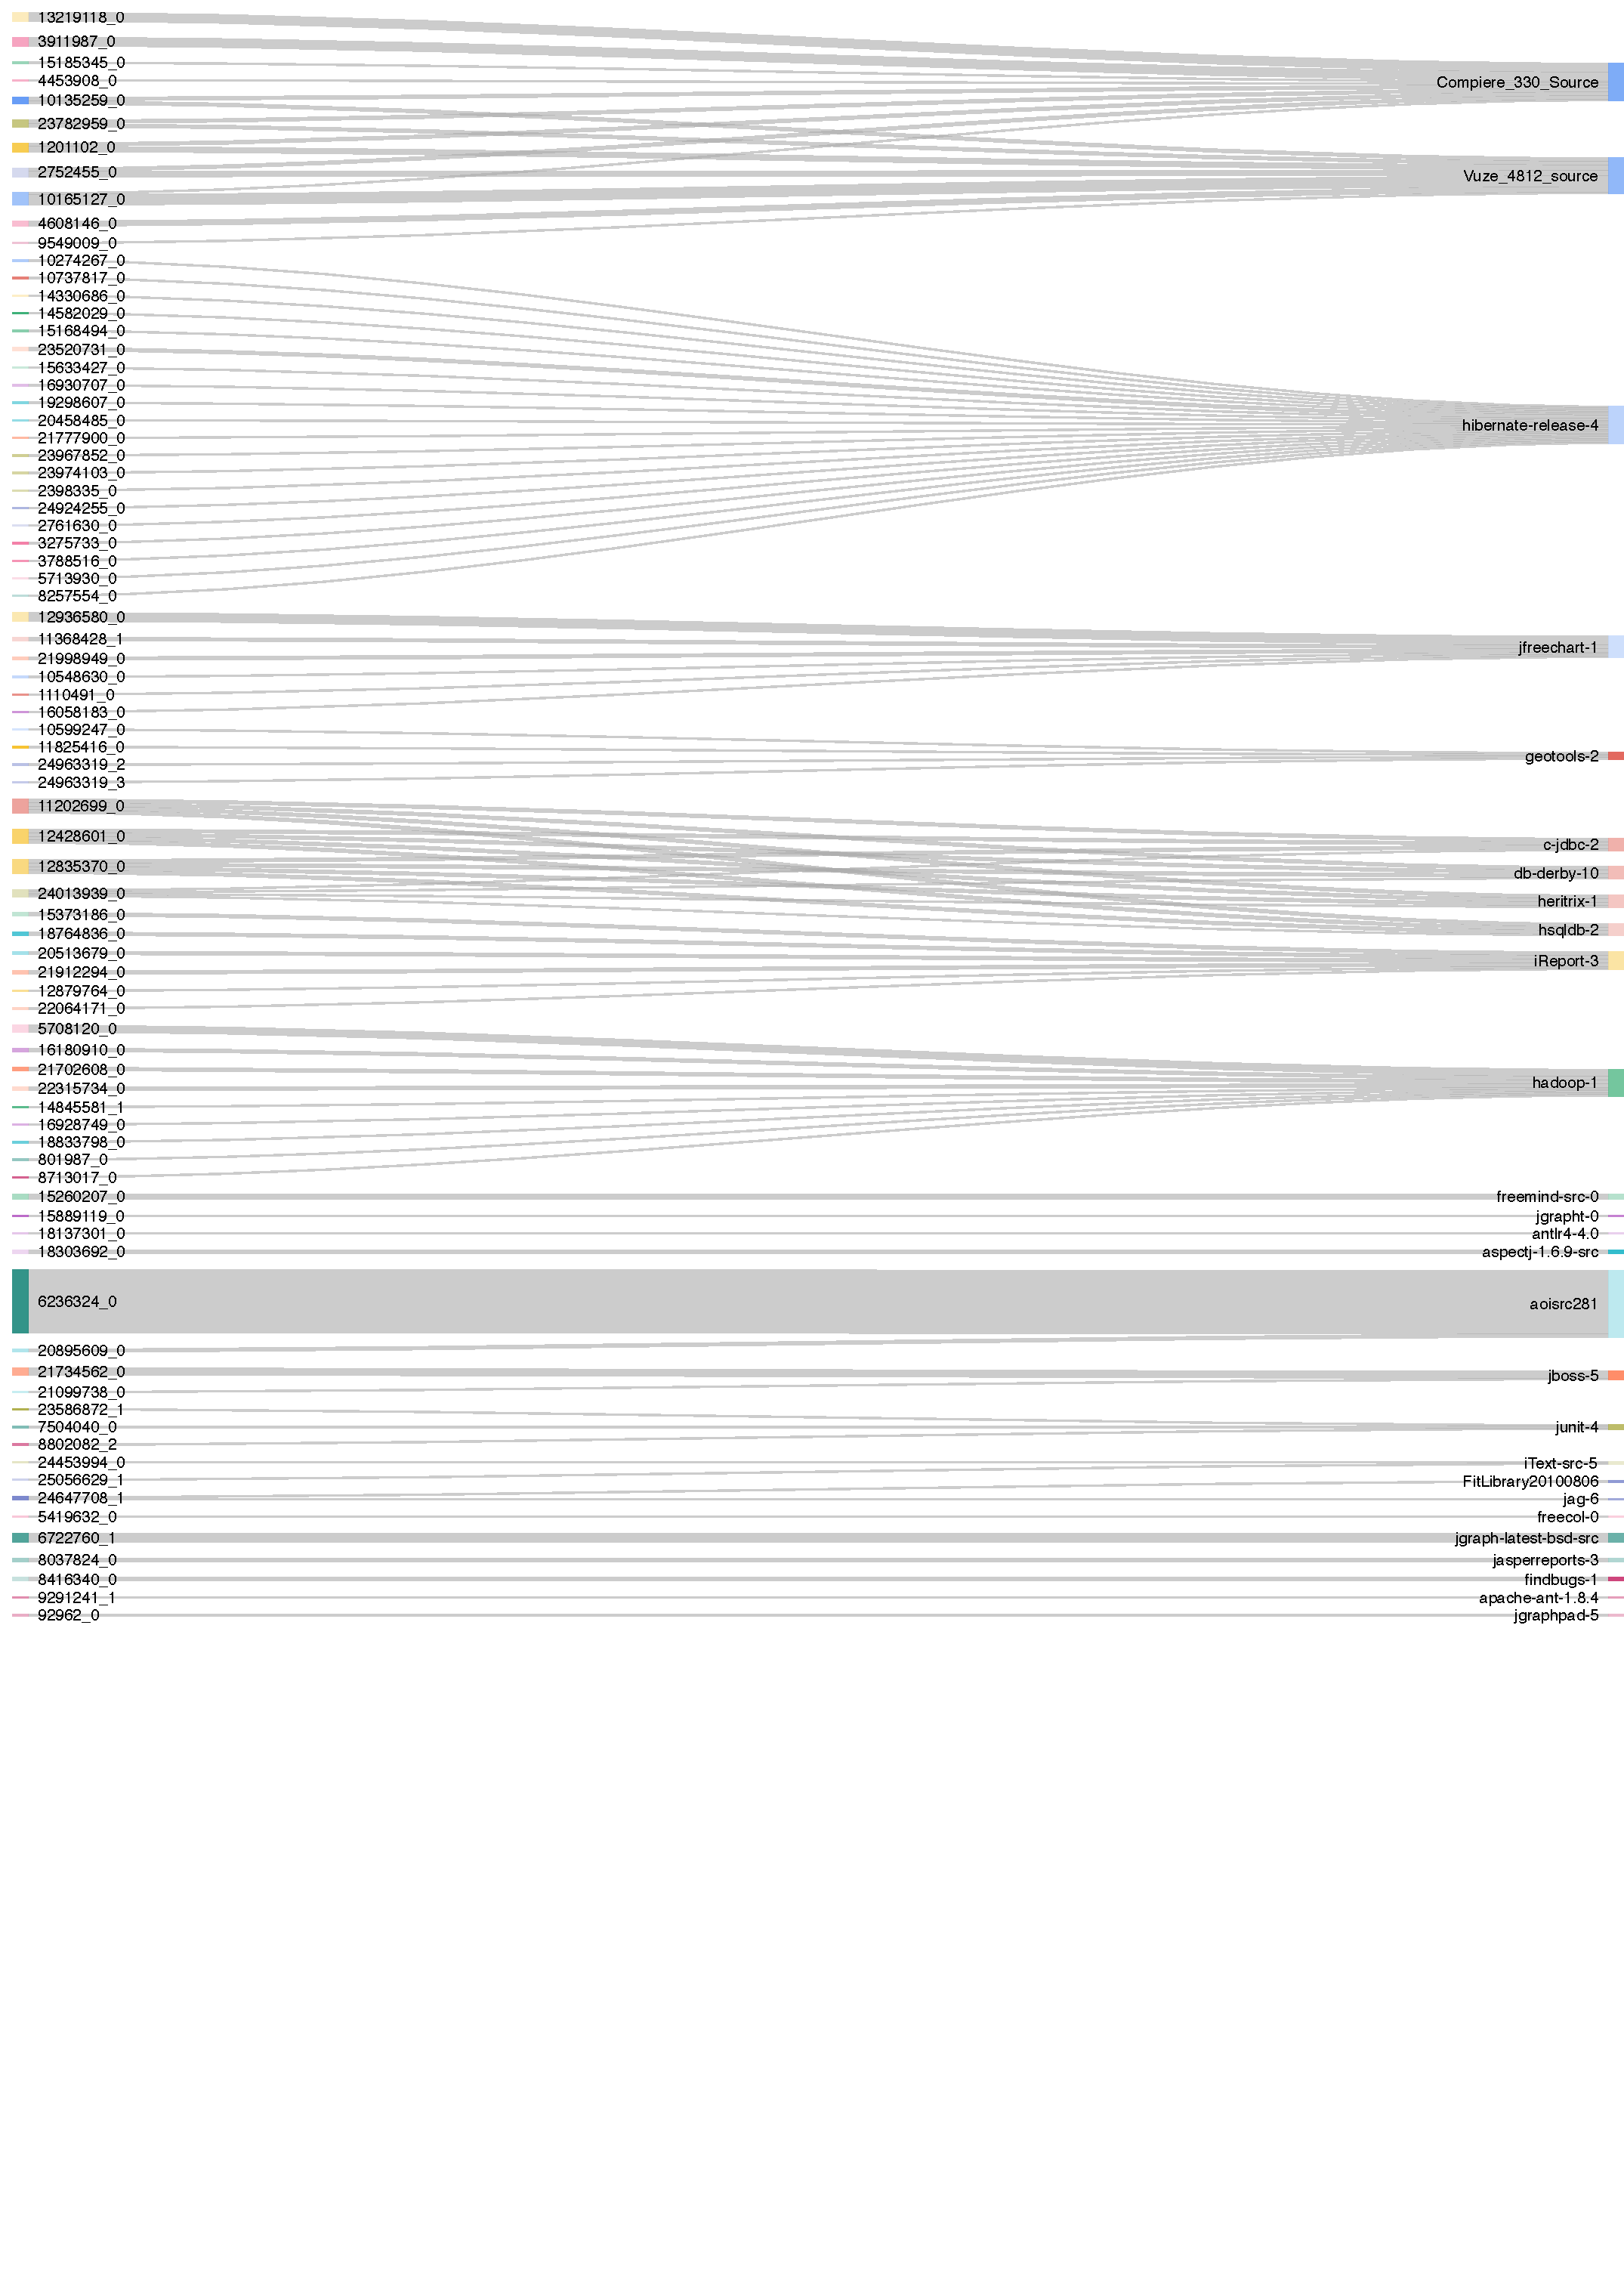
\includegraphics[width=1\linewidth]{Sankey_proj}
	\caption{Relationships between 199 true online code clone found between Stackoverflow and Qualitas projects}
	\label{fig:sankey}
\end{figure}


\newpage

\section*{Investigation of Missing A/B Clone Pairs Reported by Simian (df)}
We investigated the 41 clone pairs previously reported by Simian with default configurations and manually investigated. The 41 pairs were searched for in 4 new results sets: Simian$_{\mathrm{\textit{df}}}$, Simian$_{\mathrm{\textit{fse13}}}$, NiCad$_{\mathrm{\textit{df}}}$, NiCad$_{\mathrm{\textit{fse13}}}$. The investigation results are shown in Table \ref{tab:search}.

\begin{table}[H]
	\centering
	\caption{Results of matching the original 41 Simian(default) pairs in the pretty-printed result sets}
	\label{tab:search}
	\begin{tabular}{l|r|r}
		\hline 
		Settings & Found & Not found \\ 
		\hline 
		Simian$_{\mathrm{\textit{df}}}$  &  40 & 1* \\ 
		\hline 
		Simian$_{\mathrm{\textit{fse13}}}$ & 0 & 41  \\ 
		\hline 
		NiCad$_{\mathrm{\textit{df}}}$  & 17 & 24 \\ 
		\hline 
		NiCad$_{\mathrm{\textit{fse13}}}$ &  24 & 17 \\ 
		\hline 
	\end{tabular} 
\end{table}

The single missing Stackoverflow fragment (19051537\_0.java) (denoted by *) is one of the 11 false clones generated by Simian. It is removed from the results of the pretty-printed version because it is an outlier. The rest are missing because of different parameter settings.

\section*{Simian's Parameters}

We have carefully investigated the effects of the Simian's parameter \texttt{-balanceSquareBrackets+}. I found that it works in the expected way of handling a pair of brackets (\texttt{[},\texttt{]}) that span over multiple lines. For example, the two code fragments in Figure \ref{fig:two_frags} would match by having \texttt{-balanceSquareBrackets+} enabled.

\noindent\begin{figure}[H]
	\scriptsize
	\begin{lstlisting}[frame=single,style=base]
1           public class MagicSquare {                             public class MagicSquare2 {
2               private int[][] square;                                @private int[@
3               private boolean[] possible;                                        @][@
4               private int totalSqs;                                              @] square;@
5               private int sum;                                       private boolean[] possible;
6               private int numsquares;                                private int totalSqs;
7               public static void main ( String[] args ) {            private int sum;
8               MagicSquare m = new MagicSquare ( 3 );                 private int numsquares;
9                                                                      public static void main ( String[] args ) {
10                                                                     MagicSquare m = new MagicSquare ( 3 );
	\end{lstlisting}
	\caption{Two identical fragments with only differences in locations of the square brackets. All 7 lines are reported by Simian if \small\texttt{-balanceSquareBrackets+} \normalsize is enabled. If not, the clone pairs is reported as \newline (MagicSquare.java [3,8], MagicSquare2.java [5,10]).} 
	\label{fig:two_frags}
\end{figure}

However, the \texttt{-balanceSquareBrackets+} parameter only works on a small testing environment having toy programs or only small pairs from the full datasets. It does not work with the full complete set of 144,075 Stackoverflow fragments and Qualitas projects. Please find the summary of all the testing scenarios in Table \ref{tab:summary}. %I found that this pair is missing if I turned on \texttt{-balanceSquareBrackets+}.

\begin{table}[H]
	\caption{Simian's \texttt{-balanceSquareBrackets+} (\texttt{-bsb+}) is observed to have unpredictable behaviours when running against big datasets. $\textrm{\textit{CP}}_2$ means the reported clone(s) do not contain lines having dislocated brackets ($L_b$) (i.e. $\textrm{\textit{CP}}_2 = \textrm{\textit{CP}}_1 - L_b$).}
	\label{tab:summary}
	\centering
	\small\begin{tabular}{l|p{6cm}|c|c|c}
		\hline 
		\multirow{2}{*}{\textbf{Project 1}} & \multirow{2}{*}{\textbf{Project 2}} & \textbf{Dislocated} & \multirow{2}{*}{\textbf{-bsb+}} & \textbf{Clones pair} \\ 
		& & \textbf{brackets?} & & \textbf{reported} \\
		\hline
		\hline
		\multicolumn{5}{l}{\textit{Only run Simian against the pair}} \\
		\hline
		MagicSquare.java & MagicSquare\_exact\_copy.java & no & 0,1 & $\textrm{\textit{CP}}_1$ \\
		MagicSquare.java & MagicSquare2.java & yes & 0 & $\textrm{\textit{CP}}_2$ \\ 
		MagicSquare.java & MagicSquare2.java & yes & 1 & $\textrm{\textit{CP}}_1$ \\
		\hline
		%\hline
		%\multicolumn{5}{c}{\textit{Only run Simian against the pair}} \\
		%\hline
		stackoverflow/4298836\_0.java & Qualitas/aoisrc281/../ExprModule.java & no & 0 & $\textrm{\textit{CP}}_3$ \\ 
		stackoverflow/4298836\_0.java & Qualitas/aoisrc281/../ExprModule.java & no & 1 & $\textrm{\textit{CP}}_3$ \\ 
		stackoverflow/4533682\_1.java & Qualitas/cobertura-1/../TouchCollector.java & no & 0 & $\textrm{\textit{CP}}_4$ \\ 
		stackoverflow/4533682\_1.java & Qualitas/cobertura-1/../TouchCollector.java & no & 1 & $\textrm{\textit{CP}}_4$ \\ 
		\hline 
		\hline
		\multicolumn{5}{l}{\textit{Run Simian against the complete stackoverflow data and the project}} \\
		\hline
		stackoverflow/4298836\_0.java & Qualitas/aoisrc281/../ExprModule.java & no & 0 & $\textrm{\textit{CP}}_3$ \\ 
		\cellcolor{red!10}stackoverflow/4298836\_0.java & \cellcolor{red!10}Qualitas/aoisrc281/../ExprModule.java & \cellcolor{red!10}no & \cellcolor{red!10}1 & \cellcolor{red!10}-- \\ 
		\hline
		stackoverflow/4533682\_1.java & Qualitas/cobertura-1/../TouchCollector.java & no & 0 & $\textrm{\textit{CP}}_4$ \\ 
		\cellcolor{red!10}stackoverflow/4533682\_1.java & \cellcolor{red!10}Qualitas/cobertura-1/../TouchCollector.java & \cellcolor{red!10}no & \cellcolor{red!10}1 & \cellcolor{red!10}-- \\
		\hline 
	\end{tabular} 
\end{table}

\bibliographystyle{plain}
\bibliography{references}

\end{document}
